\chapter{ทฤษฎีเซต (Set Theory)}
\label{ch:set}

ทฤษฎีเซตใช้ระบุกลุ่มของวัตถุและความสัมพันธ์ระหว่างกลุ่มอย่างเป็นระบบ แนวคิดนี้ใช้กำหนดชนิดข้อมูล อธิบายการสืบค้นฐานข้อมูล และวิเคราะห์โครงสร้างทางคณิตศาสตร์ บทนี้อธิบายความเป็นมาของทฤษฎีเซต นิยามพื้นฐาน การดำเนินการระหว่างเซต และการประยุกต์ในวิทยาการคอมพิวเตอร์

\section{ความเป็นมาและความสำคัญของทฤษฎีเซต}
\label{sec:set-intro}
ทฤษฎีเซต (Set Theory) พัฒนาเป็นสาขาคณิตศาสตร์สมัยใหม่จากงานของแกออร์ก คันทอร์ (Georg Cantor, 1845--1918) นักคณิตศาสตร์ชาวเยอรมันในช่วงปลายศตวรรษที่ 19 งานของคันทอร์ศึกษาขนาดและชนิดของเซตอนันต์อย่างเป็นระบบ~\cite{halmos1974naive}

คันทอร์เริ่มศึกษาทฤษฎีเซตจากปัญหาเกี่ยวกับอนุกรมฟูเรียร์ (Fourier series) และความไม่ต่อเนื่องในการวิเคราะห์ทางคณิตศาสตร์ ทฤษฎีนี้ทำให้เปรียบเทียบขนาดของเซตอนันต์ได้ ตัวอย่างเช่น เซตของจำนวนเต็ม $\mathbb{Z}$ และเซตของจำนวนตรรกยะ $\mathbb{Q}$ เป็นเซตอนันต์นับได้ ขณะที่เซตของจำนวนจริง $\mathbb{R}$ เป็นเซตอนันต์นับไม่ได้ จึงมีขนาดมากกว่า

ปัจจุบันทฤษฎีเซตใช้เป็นภาษาสำหรับนิยามวัตถุ ความสัมพันธ์ และโครงสร้างในคณิตศาสตร์และวิทยาการคอมพิวเตอร์~\cite{halmos1974naive}

\subsection{ทฤษฎีเซตกับวิทยาการคอมพิวเตอร์}
แนวคิดของเซตปรากฏในชนิดข้อมูล การสืบค้นฐานข้อมูล และทฤษฎีภาษา การดำเนินการระหว่างเซตช่วยอธิบายการรวม การคัดเลือก และการเปรียบเทียบข้อมูล ตัวอย่างการนำไปใช้มีดังนี้~\cite{gersting2014structures}

\begin{enumerate}
    \item โครงสร้างข้อมูล อาร์เรย์และลิสต์เป็นลำดับข้อมูล จึงไม่ใช่เซตในความหมายทางคณิตศาสตร์ แต่ใช้เก็บตัวแทนของเซตได้เมื่อกำหนดวิธีจัดการข้อมูลซ้ำ ตารางแฮชใช้จับคู่คีย์กับตำแหน่งจัดเก็บ และโครงสร้างต้นไม้กับกราฟนิยามด้วยเซตของจุดยอดและความสัมพันธ์ระหว่างจุดยอด
    \item ระบบฐานข้อมูล ฐานข้อมูลเชิงสัมพันธ์มีพื้นฐานมาจากทฤษฎีเซตโดยตรง พีชคณิตเชิงสัมพันธ์ซึ่งเป็นพื้นฐานทางคณิตศาสตร์ของภาษาเอสคิวเอลประกอบด้วยการดำเนินการระหว่างเซต ได้แก่ ยูเนียน อินเตอร์เซกชัน ผลต่าง และผลคูณคาร์ทีเซียน
    \item ทฤษฎีภาษา ในการศึกษาภาษาการเขียนโปรแกรมและทฤษฎีการคำนวณ แนวคิดเรื่องตัวอักษร สายอักขระ และภาษา ล้วนอธิบายด้วยทฤษฎีเซต
    \item การตรวจสอบความถูกต้องของโปรแกรม การพิสูจน์ว่าโปรแกรมทำงานถูกต้องตามข้อกำหนดใช้การดำเนินการระหว่างเซตเพื่ออธิบายสถานะของโปรแกรม
    \item ทฤษฎีความน่าจะเป็น ปริภูมิตัวอย่างคือเซตของผลลัพธ์ที่เป็นไปได้ทั้งหมด และเหตุการณ์คือเซตย่อยของปริภูมิตัวอย่าง การดำเนินการระหว่างเหตุการณ์สอดคล้องกับการดำเนินการระหว่างเซต
    \item ตรรกศาสตร์และปัญญาประดิษฐ์ ระบบฐานความรู้ในปัญญาประดิษฐ์ใช้ทฤษฎีเซตในการจัดการข้อเท็จจริงและกฎเกณฑ์ การอนุมานสอดคล้องกับการดำเนินการระหว่างเซตของข้อเท็จจริง
\end{enumerate}

\begin{rem}
ในการเขียนโปรแกรม คำว่า ``เซตของตัวเลข'' อาจใช้เรียกข้อมูลในลิสต์หรืออาร์เรย์ที่มีข้อมูลซ้ำได้ แต่ในทางคณิตศาสตร์ เซตไม่มีสมาชิกซ้ำและไม่มีลำดับ เมื่อพิสูจน์สมบัติทางคณิตศาสตร์ ต้องใช้ความหมายของเซตตามนิยามนี้
\label{rem:set-programming}
\end{rem}


\section{นิยามพื้นฐานของเซต}
\label{sec:set-basics}

หัวข้อนี้อธิบายความหมายของเซต สมาชิก และวิธีเขียนเซต เนื้อหาเหล่านี้ใช้ในการนิยามการดำเนินการระหว่างเซต ความสัมพันธ์ระหว่างเซต และการพิสูจน์ทางเซตในหัวข้อถัดไป~\cite{enderton1977settheory}

ในทางคณิตศาสตร์ เซตคือกลุ่มของวัตถุที่กำหนดสมาชิกได้อย่างชัดเจน วัตถุที่อยู่ในกลุ่มเรียกว่า สมาชิก ตัวอย่างเช่น เซตของจำนวนเต็มบวกตั้งแต่ 1 ถึง 5 มีสมาชิกคือ 1, 2, 3, 4 และ 5

\subsection{นิยามของเซตและสมาชิก}
เมื่อเราจัดกลุ่มสิ่งต่าง ๆ เข้าด้วยกัน เราต้องมีวิธีบอกอย่างชัดเจนว่าสิ่งใด ``อยู่ในกลุ่ม'' หรือ ``ไม่อยู่ในกลุ่ม'' แนวคิดนี้นำไปสู่นิยามของเซตและสมาชิก ซึ่งเป็นพื้นฐานของทุกเรื่องในบทนี้ ข้อกำหนดสำคัญคือเงื่อนไขการเป็นสมาชิกต้องชัดเจนพอที่จะตัดสินได้ว่าสิ่งใดอยู่หรือไม่อยู่ในเซต โดยไม่ขึ้นกับความเห็นของผู้ตัดสิน เงื่อนไขนี้เป็นเหตุผลที่ข้อความอย่าง ``เซตของนักศึกษาที่เรียนเก่ง'' ไม่นับเป็นเซตในทางคณิตศาสตร์~\cite{lipschutz1998settheory}

\begin{definition}[เซตและสมาชิก]
\index{เซต!นิยาม}
\index{สมาชิก!นิยาม}
เซต คือกลุ่มของวัตถุที่มีสมบัติร่วมกันหรือระบุไว้อย่างชัดเจน โดยเรียกวัตถุแต่ละชิ้นว่า สมาชิก ของเซต ถ้า $a$ เป็นสมาชิกของเซต $A$ เขียนแทนด้วย $a \in A$ อ่านว่า ``$a$ เป็นสมาชิกของ $A$'' และถ้า $a$ ไม่เป็นสมาชิกของ $A$ เขียนแทนด้วย $a \notin A$
\label{def:set-membership}
\label{rem:epsilon-symbol}
\end{definition}

สัญลักษณ์ $\in$ มาจากอักษรกรีก epsilon ($\varepsilon$) ซึ่งคันทอร์นำมาใช้แทนความหมาย ``เป็นสมาชิกของ'' (element of) ข้อควรสังเกตคือความสัมพันธ์ $a \in A$ เป็นความสัมพันธ์ระหว่างวัตถุกับเซต ไม่ใช่ความสัมพันธ์ระหว่างเซตกับเซต~\cite{lipschutz1998settheory}

\begin{ex}[เซตในบริบทต่าง ๆ และสัญลักษณ์มาตรฐาน]
พิจารณาตัวอย่างต่อไปนี้ซึ่งแสดงเซตในบริบทที่แตกต่างกัน

\begin{enumerate}
    \item[(ก)] $A = \{1, 2, 3, 4, 5\}$. เซตนี้คือเซตของจำนวนเต็มบวกตั้งแต่ 1 ถึง 5 สมาชิกของ $A$ คือ 1, 2, 3, 4, 5 สังเกตว่าเราสามารถตรวจสอบได้ทันทีว่า $3 \in A$ เป็นจริง แต่ $7 \notin A$ ก็เป็นจริงเช่นกัน
    \item[(ข)] $B = \{\text{แดง}, \text{เขียว}, \text{น้ำเงิน}\}$. เซตนี้คือเซตของสีพื้นฐานในระบบสี RGB ลำดับไม่สำคัญ ดังนั้น $\{\text{แดง}, \text{เขียว}, \text{น้ำเงิน}\} = \{\text{เขียว}, \text{แดง}, \text{น้ำเงิน}\}$
    \item[(ค)] $\mathbb{N} = \{0, 1, 2, 3, \ldots\}$. เซตนี้คือเซตของจำนวนนับ (Natural Numbers) สัญลักษณ์ $\mathbb{N}$ เป็นมาตรฐาน ในตำราเล่มนี้เราจะถือว่า $\mathbb{N} = \{0, 1, 2, 3, \ldots\}$ โดยเริ่มที่ 0
    \item[(ง)] $\mathbb{Z} = \{\ldots, -2, -1, 0, 1, 2, \ldots\}$. เซตนี้คือเซตของจำนวนเต็ม (Integers) สัญลักษณ์ $\mathbb{Z}$ มาจากภาษาเยอรมัน ``Zahlen''
    \item[(จ)] $\mathbb{Q} = \left\{\frac{a}{b} \mid a, b \in \mathbb{Z}, b \neq 0\right\}$. เซตนี้คือเซตของจำนวนตรรกยะ (Rational Numbers) สัญลักษณ์ $\mathbb{Q}$ มาจาก ``quotient''
    \item[(ฉ)] $\mathbb{R}$ คือเซตของจำนวนจริง (Real Numbers) ซึ่งรวมจำนวนตรรกยะและจำนวนอตรรกยะ (irrational numbers) เช่น $\sqrt{2}$, $\pi$, $e$
\end{enumerate}
เมื่อเรากล่าวว่า $a \in A$ เรากำลังยืนยันว่าวัตถุ $a$ มีอยู่ในเซต $A$ ภายใต้การกำหนดเซตอย่างชัดเจน ข้อความนี้มีค่าความจริง (truth value) เป็นจริง (True) หรือเท็จ (False) อย่างใดอย่างหนึ่งเสมอ ไม่มีทางที่ $a \in A$ จะเป็น ``ครึ่งหนึ่งจริง'' หลักการนี้สัมพันธ์กับกฎทวิภาวะ (principle of bivalence) และสามารถเขียนในรูปกฎกีดกันกลางได้ว่า $(a \in A) \lor (a \notin A)$
\label{ex:set-examples}
\end{ex}

\begin{rem}
ความสัมพันธ์ระหว่างเซตของจำนวนต่าง ๆ เป็นดังนี้
\[
\mathbb{N} \subseteq \mathbb{Z} \subseteq \mathbb{Q} \subseteq \mathbb{R}
\]
จำนวนนับเป็นเซตย่อยของจำนวนเต็ม จำนวนเต็มเป็นเซตย่อยของจำนวนตรรกยะ และจำนวนตรรกยะเป็นเซตย่อยของจำนวนจริง ตัวอย่างเช่น $\frac{1}{2} \in \mathbb{Q}$ เป็นจริง และ $\frac{1}{2} \in \mathbb{R}$ ก็เป็นจริงด้วย แต่ $\sqrt{2} \notin \mathbb{Q}$ แต่ $\sqrt{2} \in \mathbb{R}$
\label{warn:number-sets}
\end{rem}

\begin{ex}[การตรวจสอบการเป็นสมาชิกของเซต]
จงพิจารณาว่าประโยคต่อไปนี้เป็นจริงหรือเท็จ พร้อมให้เหตุผลประกอบ
\begin{enumerate}
    \item $3 \in \{1, 2, 3, 4, 5\}$
    \item $7 \in \{1, 2, 3, 4, 5\}$
    \item $\sqrt{2} \in \mathbb{Q}$
    \item $\sqrt{2} \in \mathbb{R}$
    \item $0.75 \in \mathbb{Q}$
    \item $0.\overline{3} \in \mathbb{Q}$
\end{enumerate}
\end{ex}

\begin{solution}
\begin{align*}
3 \in \{1,2,3,4,5\} &\equiv \text{T}\\
7 \in \{1,2,3,4,5\} &\equiv \text{F}\\
\sqrt{2} \in \mathbb{Q} &\equiv \text{F} \quad (\sqrt{2} \text{ เป็นจำนวนอตรรกยะ})\\
\sqrt{2} \in \mathbb{R} &\equiv \text{T}\\
0.75 \in \mathbb{Q} &\equiv \text{T} \quad (0.75 = \tfrac{3}{4})\\
0.\overline{3} \in \mathbb{Q} &\equiv \text{T} \quad (0.\overline{3} = \tfrac{1}{3})
\end{align*}
\solhere
\end{solution}

\subsection{วิธีการเขียนเซต}
เซตเดียวกันสามารถเขียนแทนได้มากกว่าหนึ่งวิธี การเลือกวิธีเขียนขึ้นอยู่กับจำนวนสมาชิกและลักษณะของเซต ถ้าเซตมีสมาชิกไม่มากและระบุได้ครบทุกตัว การเขียนไล่สมาชิกออกมาโดยตรงจะชัดเจนที่สุด แต่ถ้าเซตมีสมาชิกจำนวนมากหรือมีจำนวนไม่สิ้นสุดจนไล่ไม่หมด เราจะอธิบายเซตด้วยเงื่อนไขที่สมาชิกทุกตัวต้องมีร่วมกันแทน ด้วยเหตุนี้ วิธีเขียนเซตที่ใช้กันจึงมี 2 แบบหลัก ดังนี้~\cite{rosen2019discrete}

\begin{enumerate}
    \item \textbf{แจกแจงสมาชิก (Roster Method)} คือการเขียนสมาชิกทั้งหมดภายในวงเล็บปีกกา $\{\}$ โดยคั่นด้วยเครื่องหมายจุลภาค วิธีนี้เหมาะกับเซตที่มีจำนวนสมาชิกน้อยและสามารถระบุได้ทั้งหมด

    \begin{enumerate}[leftmargin=2.5em,label=\arabic*.]
        \item $A = \{1, 2, 3\}$ แสดงเซตที่มีสมาชิกสามตัว $B = \{a, e, i, o, u\}$ แสดงเซตของสระในภาษาอังกฤษ สังเกตว่าลำดับไม่สำคัญ $\{a, e, i, o, u\} = \{e, a, i, o, u\}$ และไม่มีสมาชิกซ้ำ $\{1, 1, 2, 2, 3\} = \{1, 2, 3\}$
        \item \textbf{การใช้ ... (ellipsis):} เมื่อเซตมีสมาชิกมากแต่มีรูปแบบที่ชัดเจน เช่น $\{1, 2, 3, \ldots, 100\}$ แสดงเซตของจำนวนเต็มตั้งแต่ 1 ถึง 100 ข้อควรระวังคือต้องเขียนสมาชิกอย่างน้อย 2 ตัวก่อนจุดไข่ปลา เพื่อให้ผู้อ่านเข้าใจรูปแบบ
    \end{enumerate}

    \item \textbf{แจกแจงโดยกำหนดสมบัติ (Set-builder Notation)} คือการเขียนในรูป $\{x \mid \text{เงื่อนไขที่ } x \text{ ต้องสอดคล้อง}\}$ วิธีนี้เหมาะกับเซตที่มีจำนวนสมาชิกมากหรืออนันต์ พิจารณาตัวอย่างต่อไปนี้
    \begin{enumerate}[leftmargin=2.5em,label=\arabic*.]
        \item $A = \{x \in \mathbb{Z} \mid x > 0\}$. เซตนี้คือเซตของจำนวนเต็มบวก เขียนแบบย่อได้เป็น $\mathbb{Z}^+$
        \item $B = \{n^2 \mid n \in \mathbb{N} \text{ และ } n < 5\} = \{0, 1, 4, 9, 16\}$. สมาชิกของเซตนี้คือกำลังสองของจำนวนนับที่น้อยกว่า 5
        \item $E = \{x \in \mathbb{Z} \mid x \text{ หารด้วย } 2 \text{ ลงตัว}\} = 2\mathbb{Z}$. เซตนี้คือเซตของจำนวนคู่
        \item $O = \{x \in \mathbb{Z} \mid x \text{ หารด้วย } 2 \text{ ไม่ลงตัว}\}$. เซตนี้คือเซตของจำนวนคี่
        \item $C = \{x \in \mathbb{R} \mid x^2 - 5x + 6 = 0\} = \{2, 3\}$. เซตนี้คือเซตของคำตอบของสมการ $x^2 - 5x + 6 = 0$
        \item $D = \{x \in \mathbb{R} \mid x^2 + 1 = 0\} = \emptyset$. ไม่มีจำนวนจริงที่ยกกำลังสองแล้วบวก 1 ได้ศูนย์
    \end{enumerate}
\end{enumerate}

\begin{rem}
เซตมีสมบัติสำคัญสองประการดังนี้
\begin{enumerate}
    \item ไม่มีลำดับ (Unordered) คือลำดับของสมาชิกไม่สำคัญ $\{1, 2\} = \{2, 1\}$ หากต้องการลำดับ ต้องใช้ tuple หรือ sequence แทน
    \item ไม่มีสมาชิกซ้ำ (No Duplicates) คือ $\{1, 1, 2\} = \{1, 2\}$ หากต้องซ้ำ ต้องใช้ multiset หรือ list แทน
\end{enumerate}
\end{rem}


\subsection{เซตพิเศษ}
ในบรรดาเซตทั้งหมด มีบางเซตที่ปรากฏซ้ำ ๆ ในเกือบทุกหัวข้อจนคณิตศาสตร์กำหนดชื่อและสัญลักษณ์เฉพาะไว้ให้ การรู้จักเซตเหล่านี้ช่วยให้เขียนนิยามและพิสูจน์ได้กระชับและสื่อความตรงกัน หัวข้อนี้จะแนะนำเซตพิเศษที่ใช้บ่อยที่สุด ได้แก่ เซตว่างที่ไม่มีสมาชิกเลย เอกภพสัมพัทธ์ที่กำหนดขอบเขตของสิ่งที่พิจารณา และเซตของจำนวนมาตรฐานที่ใช้อ้างอิงตลอดทั้งเล่ม~\cite{epp2019discrete}

\begin{definition}[เซตพิเศษ]
\index{เซตพิเศษ!นิยาม}
เซตพิเศษที่ใช้บ่อย ได้แก่
\begin{enumerate}
    \item เซตว่าง เขียนแทนด้วย $\emptyset$ หรือ $\{\quad\}$ คือเซตที่ไม่มีสมาชิก
    \item เซตที่มีสมาชิกตัวเดียว คือเซตที่มีสมาชิกเพียงตัวเดียว เช่น $\{5\}$, $\{a\}$, $\{\emptyset\}$
    \item เอกภพสัมพัทธ์ เขียนแทนด้วย $U$ คือเซตของสมาชิกทั้งหมดที่พิจารณาในบริบทหนึ่ง
    \item เซตจำกัด คือเซตที่มีจำนวนสมาชิกจำกัด ส่วน เซตอนันต์ คือเซตที่มีจำนวนสมาชิกไม่สิ้นสุด เช่น $\mathbb{N}$, $\mathbb{Z}$, $\mathbb{Q}$, $\mathbb{R}$
\end{enumerate}
\label{def:special-sets}
\end{definition}

เซตว่างมีสมบัติที่ควรจำคือเป็นเซตย่อยของทุกเซต เขียนได้ว่า $\emptyset \subseteq A$ สำหรับทุกเซต $A$ เหตุผลคือข้อความ ``สมาชิกทุกตัวของ $\emptyset$ อยู่ใน $A$'' เป็นจริงโดยปริยาย (vacuous truth) เพราะ $\emptyset$ ไม่มีสมาชิกที่จะขัดกับเงื่อนไขได้ ส่วนเอกภพสัมพัทธ์ $U$ ทำหน้าที่เป็นกรอบกำหนดขอบเขตของสมาชิกที่นำมาพิจารณา การเลือก $U$ ต่างกันจะส่งผลต่อการดำเนินการบางอย่าง เช่น คอมพลีเมนต์ ดังจะเห็นในหัวข้อถัดไป

\begin{rem}[ข้อสังเกตเกี่ยวกับเซตว่าง]
\index{เซตว่าง!ข้อสังเกต}
ความเข้าใจผิดที่พบบ่อยเกี่ยวกับเซตว่างมีสองเรื่องดังนี้
\begin{enumerate}[label=\textbf{\arabic*.},leftmargin=1.5em,itemsep=0.3em]
    \item \textbf{ความแตกต่างของสัญลักษณ์:} $\emptyset$ คือเซตที่ไม่มีสมาชิกเลย ($|\emptyset| = 0$) แต่ $\{\emptyset\}$ คือเซตที่มีสมาชิก 1 ตัว คือ $\emptyset$ ($|\{\emptyset\}| = 1$) ดังนั้น $\emptyset \neq \{\emptyset\} \neq \{\{\emptyset\}\}$
    \item \textbf{ความแตกต่างระหว่างสมาชิกกับเซตย่อย:} $\emptyset \in \{\emptyset\}$ เป็นจริง เพราะ $\emptyset$ เป็นสมาชิกของ $\{\emptyset\}$ และ $\emptyset \subseteq \{\emptyset\}$ ก็เป็นจริงด้วย (เซตว่างเป็นเซตย่อยของทุกเซต) แสดงว่า $\in$ (เป็นสมาชิก) และ $\subseteq$ (เป็นเซตย่อย) เป็นความสัมพันธ์ที่ต่างกัน แต่สามารถเป็นจริงทั้งคู่พร้อมกันได้
\end{enumerate}
\end{rem}

\begin{ex}[การแยกความแตกต่างระหว่างการเป็นสมาชิกกับการเป็นเซตย่อย]
จงพิจารณาว่าข้อความต่อไปนี้เป็นจริงหรือเท็จ พร้อมให้เหตุผล
\begin{enumerate}
    \item $1 \in \{1, 2, 3\}$
    \item $\{1\} \in \{1, 2, 3\}$
    \item $\{1\} \subseteq \{1, 2, 3\}$
    \item $\emptyset \subseteq \{1, 2, 3\}$
    \item $\emptyset \in \{1, 2, 3\}$
\end{enumerate}
\end{ex}
\begin{solution}
\begin{align*}
1 \in \{1,2,3\} &\equiv \text{T} \quad (1 \text{ เป็นสมาชิก})\\
\{1\} \in \{1,2,3\} &\equiv \text{F} \quad (\{1\} \text{ ไม่ใช่สมาชิก})\\
\{1\} \subseteq \{1,2,3\} &\equiv \text{T} \quad (\text{ทุกสมาชิกของ } \{1\} \text{ อยู่ใน } \{1,2,3\})\\
\emptyset \subseteq \{1,2,3\} &\equiv \text{T} \quad (\text{เซตว่างเป็นเซตย่อยของทุกเซต})\\
\emptyset \in \{1,2,3\} &\equiv \text{F}
\end{align*}
หลักที่ใช้แยกสองความสัมพันธ์นี้คือ $\in$ เปรียบเทียบวัตถุกับเซต ส่วน $\subseteq$ เปรียบเทียบเซตกับเซต ข้อ 2 จึงเป็นเท็จ เพราะสมาชิกของ $\{1,2,3\}$ คือจำนวน 1, 2 และ 3 ไม่ใช่เซต $\{1\}$ ขณะที่ข้อ 3 เป็นจริงเพราะสมาชิกทุกตัวของ $\{1\}$ อยู่ใน $\{1,2,3\}$ ทั้งสองความสัมพันธ์เป็นจริงพร้อมกันได้ในบางกรณี เช่น $1 \in \{1\}$ และ $\{1\} \subseteq \{1\}$ \solhere
\end{solution}

\section{ความสัมพันธ์ระหว่างเซต}

เมื่อมีเซตสองเซต คำถามพื้นฐานที่ตามมาคือเซตทั้งสองเกี่ยวข้องกันอย่างไร สมาชิกของเซตหนึ่งอยู่ในอีกเซตหนึ่งครบทุกตัวหรือไม่ และเซตทั้งสองถือว่าเท่ากันเมื่อใด หัวข้อนี้ตอบคำถามเหล่านั้นด้วยแนวคิดเรื่องเซตย่อยและความเท่ากันของเซต ซึ่งเป็นเครื่องมือที่ใช้พิสูจน์ผลลัพธ์ทางทฤษฎีเซตแทบทุกข้อในหัวข้อถัดไป~\cite{johnsonbaugh2016discrete}

\subsection{เซตย่อย (Subset) และเซตย่อยแท้ (Proper Subset)}
นิยามเซตย่อยใช้เป็นพื้นฐานของการพิสูจน์ทางเซต เมื่อต้องการพิสูจน์ว่า $A \subseteq B$ ให้สมมติว่า $x \in A$ แล้วแสดงว่า $x \in B$ วิธีนี้เรียกว่าการพิสูจน์ตรง (Direct Proof) สำหรับเซตย่อย ส่วนเซตย่อยแท้เพิ่มเงื่อนไขว่าต้องมีสมาชิกใน $B$ อย่างน้อยหนึ่งตัวที่ไม่อยู่ใน $A$ การแยกสองแนวคิดนี้ทำให้ระบุได้ว่าเซตหนึ่งเท่ากับหรือเป็นเซตย่อยแท้ของอีกเซตหนึ่ง~\cite{halmos1974naive}

\begin{definition}[เซตย่อยและเซตย่อยแท้]
\index{เซตย่อย!นิยาม}
\index{เซตย่อยแท้!นิยาม}
เซต $A$ เป็นเซตย่อยของเซต $B$ เขียนแทนด้วย $A \subseteq B$ ก็ต่อเมื่อทุกสมาชิกของ $A$ เป็นสมาชิกของ $B$ กล่าวคือ $\forall x, (x \in A \rightarrow x \in B)$ นอกจากนี้ $\emptyset \subseteq A$ และ $A \subseteq A$ สำหรับทุกเซต $A$ เซต $A$ และ $B$ เท่ากันก็ต่อเมื่อ $A \subseteq B$ และ $B \subseteq A$ ส่วน $A \subseteq B$ และ $B \not\subseteq A$ หมายถึง $A \subsetneq B$ หรือ $A$ เป็นเซตย่อยแท้ของ $B$ ตัวอย่างเช่น $\{1, 2\} \subsetneq \{1, 2, 3\}$ เพราะ $\{1, 2\} \subseteq \{1, 2, 3\}$ แต่ $\{1, 2, 3\} \not\subseteq \{1, 2\}$
\end{definition}

\begin{ex}[การตรวจสอบความเป็นเซตย่อย]
จงพิจารณาว่าข้อความต่อไปนี้เป็นจริงหรือเท็จ พร้อมให้เหตุผล
\begin{enumerate}
    \item $\{1, 2\} \subseteq \{1, 2, 3\}$
    \item $\mathbb{N} \subseteq \mathbb{Z} \subseteq \mathbb{Q} \subseteq \mathbb{R}$
    \item $\emptyset \subseteq \{1, 2\}$
    \item $\{1, 2\} \not\subseteq \{2, 3\}$
\end{enumerate}
\end{ex}

\begin{solution}
ตรวจทีละข้อโดยไล่ดูว่าสมาชิกทุกตัวของเซตทางซ้ายอยู่ในเซตทางขวาหรือไม่
\begin{align*}
\{1,2\} \subseteq \{1,2,3\} &\equiv \text{T} \quad (1,2 \in \{1,2,3\})\\
\mathbb{N} \subseteq \mathbb{Z} \subseteq \mathbb{Q} \subseteq \mathbb{R} &\equiv \text{T}\\
\emptyset \subseteq \{1,2\} &\equiv \text{T} \quad (\text{เซตว่างเป็นเซตย่อยของทุกเซต})\\
\{1,2\} \not\subseteq \{2,3\} &\equiv \text{T} \quad (1 \in \{1,2\} \text{ แต่ } 1 \notin \{2,3\})
\end{align*}
ข้อ 4 ต้องอ่านให้ตรงว่าข้อความที่ถามคือ ``$\{1,2\}$ ไม่เป็นเซตย่อยของ $\{2,3\}$'' ซึ่งเป็นจริง เพราะพบสมาชิกอย่างน้อยหนึ่งตัวที่ขัดเงื่อนไข การหักล้างความเป็นเซตย่อยจึงต้องการตัวอย่างค้านเพียงตัวเดียวเท่านั้น \solhere
\end{solution}

\begin{principle}
ในการพิสูจน์ว่า $A = B$ เราต้องพิสูจน์ทั้ง $A \subseteq B$ และ $B \subseteq A$ นั่นคือต้องแสดงสองข้อ ข้อแรก ทุก $x \in A \Rightarrow x \in B$ (แสดง $A \subseteq B$) และข้อที่สอง ทุก $x \in B \Rightarrow x \in A$ ซึ่งแสดงว่า $B \subseteq A$ วิธีนี้เรียกว่าการพิสูจน์ด้วยการบรรจุสองทาง (double inclusion) เป็นเทคนิคมาตรฐานในการพิสูจน์ความเท่ากันของเซต
\label{thrm:double-inclusion}
\end{principle}

\begin{ex}[การพิสูจน์กฎการแจกแจงของเซต]
พิสูจน์ว่า $A \cap (B \cup C) = (A \cap B) \cup (A \cap C)$ (กฎการแจกแจง)
\end{ex}
\begin{solution}
พิสูจน์แบบสมาชิก โดยแสดงว่า $x$ อยู่ในเซตด้านซ้ายก็ต่อเมื่ออยู่ในเซตด้านขวา
\[
x \in A \cap (B \cup C) \Leftrightarrow x \in A \ \land\ (x \in B \lor x \in C)
\]
\[
\Leftrightarrow (x \in A \land x \in B) \lor (x \in A \land x \in C) \quad (\text{กฎแจกแจงตรรกศาสตร์})
\]
\[
\Leftrightarrow x \in (A \cap B) \ \lor\ x \in (A \cap C)
\]
\[
\Leftrightarrow x \in (A \cap B) \cup (A \cap C)
\]
$\therefore A \cap (B \cup C) = (A \cap B) \cup (A \cap C)$ \solhere
\end{solution}

\section{การดำเนินการระหว่างเซต (Set Operations)}

การดำเนินการระหว่างเซตเป็นเครื่องมือพื้นฐานในการสร้างเซตใหม่จากเซตที่มีอยู่ หัวข้อนี้ศึกษาการดำเนินการสี่อย่างหลัก ได้แก่ ยูเนียน ($\cup$) อินเตอร์เซกชัน ($\cap$) ผลต่าง ($-$) และคอมพลีเมนต์ ($^c$) การดำเนินการทั้งสี่มีคู่ขนานโดยตรงกับตัวเชื่อมทางตรรกศาสตร์ที่ศึกษาในบทที่ 1 คือ OR, AND, และ NOT ความสอดคล้องนี้ทำให้พิสูจน์สมบัติของเซตด้วยตารางค่าความจริงได้~\cite{enderton1977settheory}

\subsection{ยูเนียน (Union)}
ยูเนียนเป็นการรวมสมาชิกของสองเซตเป็นเซตเดียว สมาชิกที่อยู่ทั้งสองเซตปรากฏในผลลัพธ์เพียงครั้งเดียว เพราะเซตไม่นับสมาชิกซ้ำ ดังนั้นจำนวนสมาชิกของยูเนียนจึงไม่จำเป็นต้องเท่ากับผลบวกของจำนวนสมาชิกของทั้งสองเซต~\cite{lipschutz1998settheory}

\begin{definition}[ยูเนียน]
\index{ยูเนียน!นิยาม}
ยูเนียน ของเซต $A$ และ $B$ เขียนแทนด้วย $A \cup B$ คือเซตที่ประกอบด้วยสมาชิกที่อยู่ใน $A$ หรืออยู่ใน $B$ หรืออยู่ทั้งสองเซต นั่นคือ
\[ A \cup B = \{x \mid x \in A \text{ หรือ } x \in B\} \]
\label{def:union}
\end{definition}

สมาชิกจะเข้ามาอยู่ในผลลัพธ์ก็ต่อเมื่อมันอยู่ใน $A$ หรืออยู่ใน $B$ อย่างน้อยหนึ่งเซต และสมาชิกที่อยู่ทั้งสองเซตจะปรากฏในผลลัพธ์เพียงครั้งเดียว เพราะเซตไม่มีสมาชิกซ้ำ ยูเนียนมีสมบัติสำคัญดังนี้
\begin{enumerate}
    \item $A \cup A = A$ (กฎนิจพล)
    \item $A \cup \emptyset = A$ (กฎเอกลักษณ์)
    \item $A \cup U = U$ (กฎครอบงำ)
    \item $A \cup B = B \cup A$ (กฎการสลับที่)
    \item $(A \cup B) \cup C = A \cup (B \cup C)$ (กฎการเปลี่ยนหมู่)
\end{enumerate}
นอกจากนี้ยังได้ว่า $A \subseteq A \cup B$ และ $B \subseteq A \cup B$ สำหรับทุกเซต $A$, $B$, $C$

\begin{ex}[การหายูเนียนในกรณีต่าง ๆ]
จงหาผลของยูเนียนต่อไปนี้ พร้อมระบุสมบัติที่แต่ละข้อแสดงให้เห็น
\begin{enumerate}
    \item $\{1, 2\} \cup \{2, 3\}$
    \item $\{1, 2\} \cup \emptyset$
    \item $\{x \mid x \text{ เป็นจำนวนคู่}\} \cup \{x \mid x \text{ เป็นจำนวนคี่}\}$
    \item $A \cup A$ และ $A \cup B$ เทียบกับ $B \cup A$
\end{enumerate}
\end{ex}
\begin{solution}
\begin{align*}
\{1,2\} \cup \{2,3\} &= \{1,2,3\} \quad (2 \text{ อยู่ทั้งสองเซต ปรากฏครั้งเดียว})\\
\{1,2\} \cup \emptyset &= \{1,2\} \quad (\text{กฎเอกลักษณ์})\\
\{x \mid x \text{ คู่}\} \cup \{x \mid x \text{ คี่}\} &= \mathbb{Z}\\
A \cup A &= A \quad (\text{กฎนิจพล})\\
A \cup B &= B \cup A \quad (\text{กฎการสลับที่})
\end{align*}
\solhere
\end{solution}

\begin{ex}[การหายูเนียนของเซต]
กำหนดให้ $A = \{1, 2, 3, 4\}$ และ $B = \{3, 4, 5, 6\}$ จงหา $A \cup B$
\end{ex}

\begin{solution}
รวมสมาชิกที่อยู่ใน $A$ หรือ $B$ โดยนับสมาชิกที่ซ้ำเพียงครั้งเดียว
\begin{align*}
A \cup B &= \{1,2,3,4\} \cup \{3,4,5,6\}\\
         &= \{1,2,3,4,5,6\}
\end{align*}
สมาชิก 3 และ 4 อยู่ทั้งสองเซตแต่ปรากฏในผลลัพธ์เพียงครั้งเดียว ตามนิยามของเซตที่ไม่มีสมาชิกซ้ำ
\label{ex:union-step-by-step}
\solhere
\end{solution}

\begin{figure}[H]
    \centering
    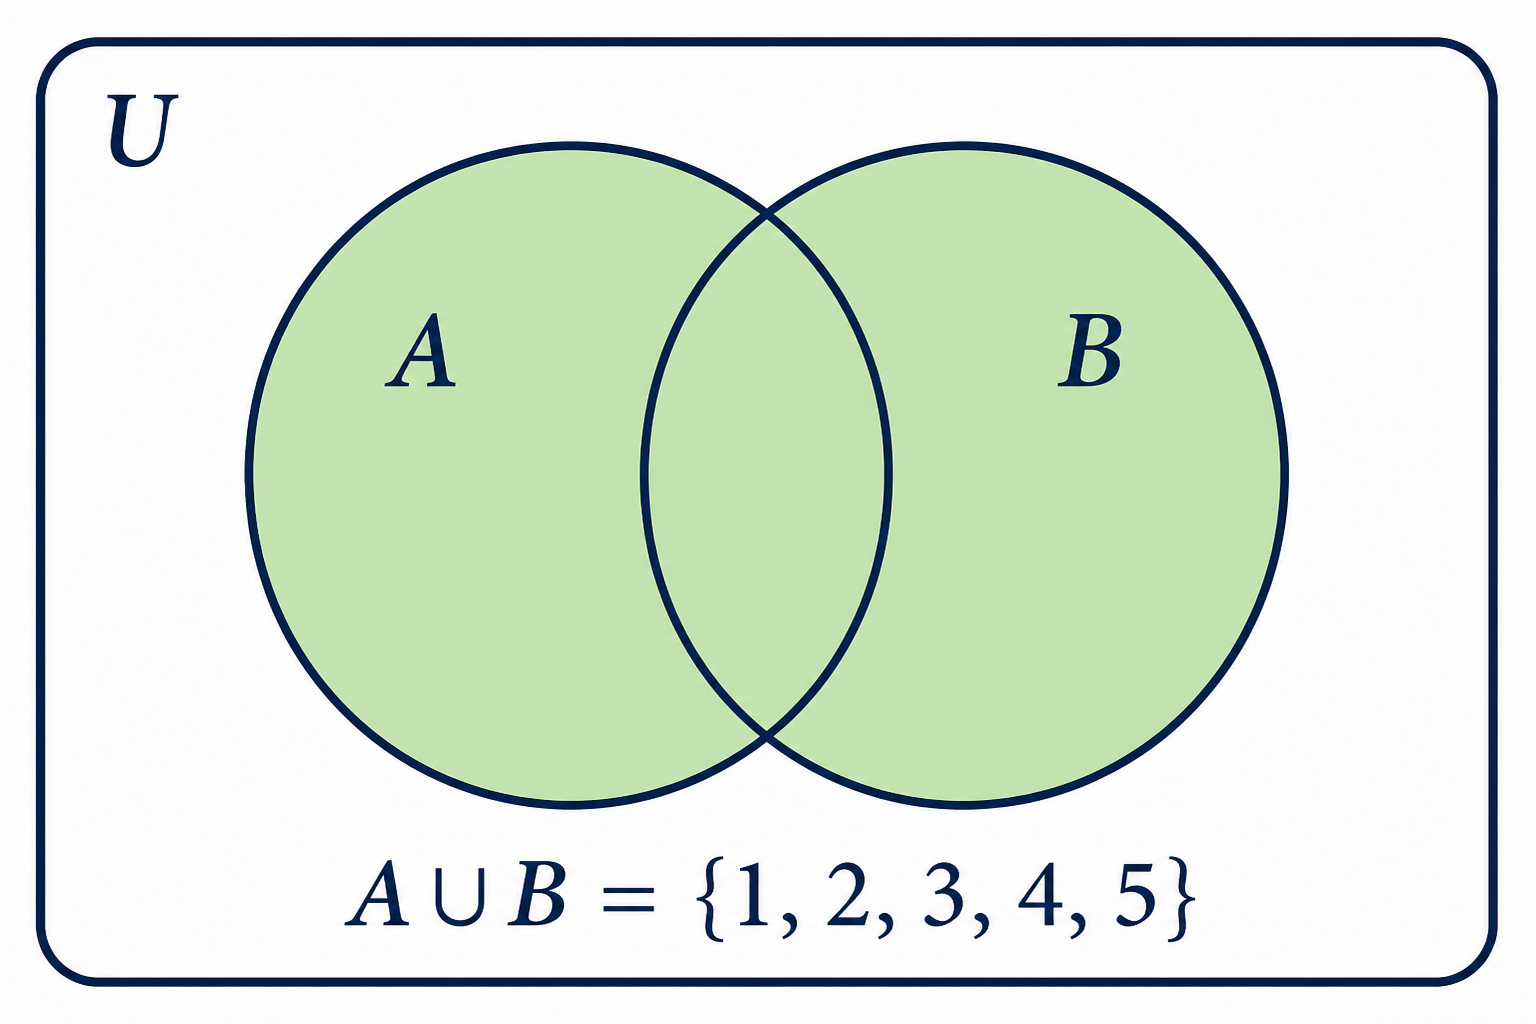
\includegraphics[width=0.65\textwidth]{Figures/png_ready/10-venn-union-generated.png}
    \caption{แผนภาพเวนน์แสดงการดำเนินการยูเนียน $A \cup B$}
    \label{fig:venn-union}
\end{figure}

รูปที่ \ref{fig:venn-union} แสดงแผนภาพเวนน์ของยูเนียน $A \cup B$ โดยพื้นที่ที่แรเงาคือผลลัพธ์ของการรวมเซต $A$ และเซต $B$

\subsection{อินเตอร์เซกชัน (Intersection)}
อินเตอร์เซกชัน (Intersection) คือเซตของสมาชิกที่อยู่ในทั้งสองเซต การที่ $x \in A \cap B$ หมายความว่า $x$ เป็นสมาชิกของ $A$ และเป็นสมาชิกของ $B$ ในทางตรรกศาสตร์สอดคล้องกับตัวเชื่อม ``และ'' (AND) ถ้า $A \cap B = \emptyset$ จะเรียก $A$ และ $B$ ว่า \textbf{เซตไม่มีสมาชิกร่วม (Disjoint Sets)}~\cite{rosen2019discrete}

\begin{definition}[อินเตอร์เซกชัน]
\index{อินเตอร์เซกชัน!นิยาม}
อินเตอร์เซกชัน ของเซต $A$ และ $B$ เขียนแทนด้วย $A \cap B$ คือเซตที่ประกอบด้วยสมาชิกที่อยู่ทั้งใน $A$ และใน $B$ พร้อมกัน นั่นคือ
\[ A \cap B = \{x \mid x \in A \text{ และ } x \in B\} \]
\end{definition}

อินเตอร์เซกชันมีสมบัติสำคัญดังนี้
\begin{enumerate}
    \item $A \cap A = A$ (กฎนิจพล)
    \item $A \cap \emptyset = \emptyset$ (กฎครอบงำ)
    \item $A \cap U = A$ (กฎเอกลักษณ์)
    \item $A \cap B = B \cap A$ (กฎการสลับที่)
    \item $(A \cap B) \cap C = A \cap (B \cap C)$ (กฎการเปลี่ยนหมู่)
\end{enumerate}
นอกจากนี้ยังได้ว่า $A \cap B \subseteq A$ และ $A \cap B \subseteq B$

\begin{ex}[การหาอินเตอร์เซกชันในกรณีต่าง ๆ]
จงหาผลของอินเตอร์เซกชันต่อไปนี้ พร้อมระบุว่าคู่ใดเป็นเซตไม่มีสมาชิกร่วม
\begin{enumerate}
    \item $\{1, 2\} \cap \{2, 3\}$
    \item $\{1, 2\} \cap \{3, 4\}$
    \item $\mathbb{Z} \cap \mathbb{R}$
    \item $\{x \mid x \text{ เป็นจำนวนคู่}\} \cap \{x \mid x \text{ เป็นจำนวนคี่}\}$
\end{enumerate}
\end{ex}
\begin{solution}
\begin{align*}
\{1,2\} \cap \{2,3\} &= \{2\} \quad (2 \text{ อยู่ทั้งสองเซต})\\
\{1,2\} \cap \{3,4\} &= \emptyset \quad (\text{เซตไม่มีสมาชิกร่วม})\\
\mathbb{Z} \cap \mathbb{R} &= \mathbb{Z} \quad (\mathbb{Z} \subseteq \mathbb{R})\\
\{x \mid x \text{ คู่}\} \cap \{x \mid x \text{ คี่}\} &= \emptyset
\end{align*}
\solhere
\end{solution}

\begin{figure}[H]
    \centering
    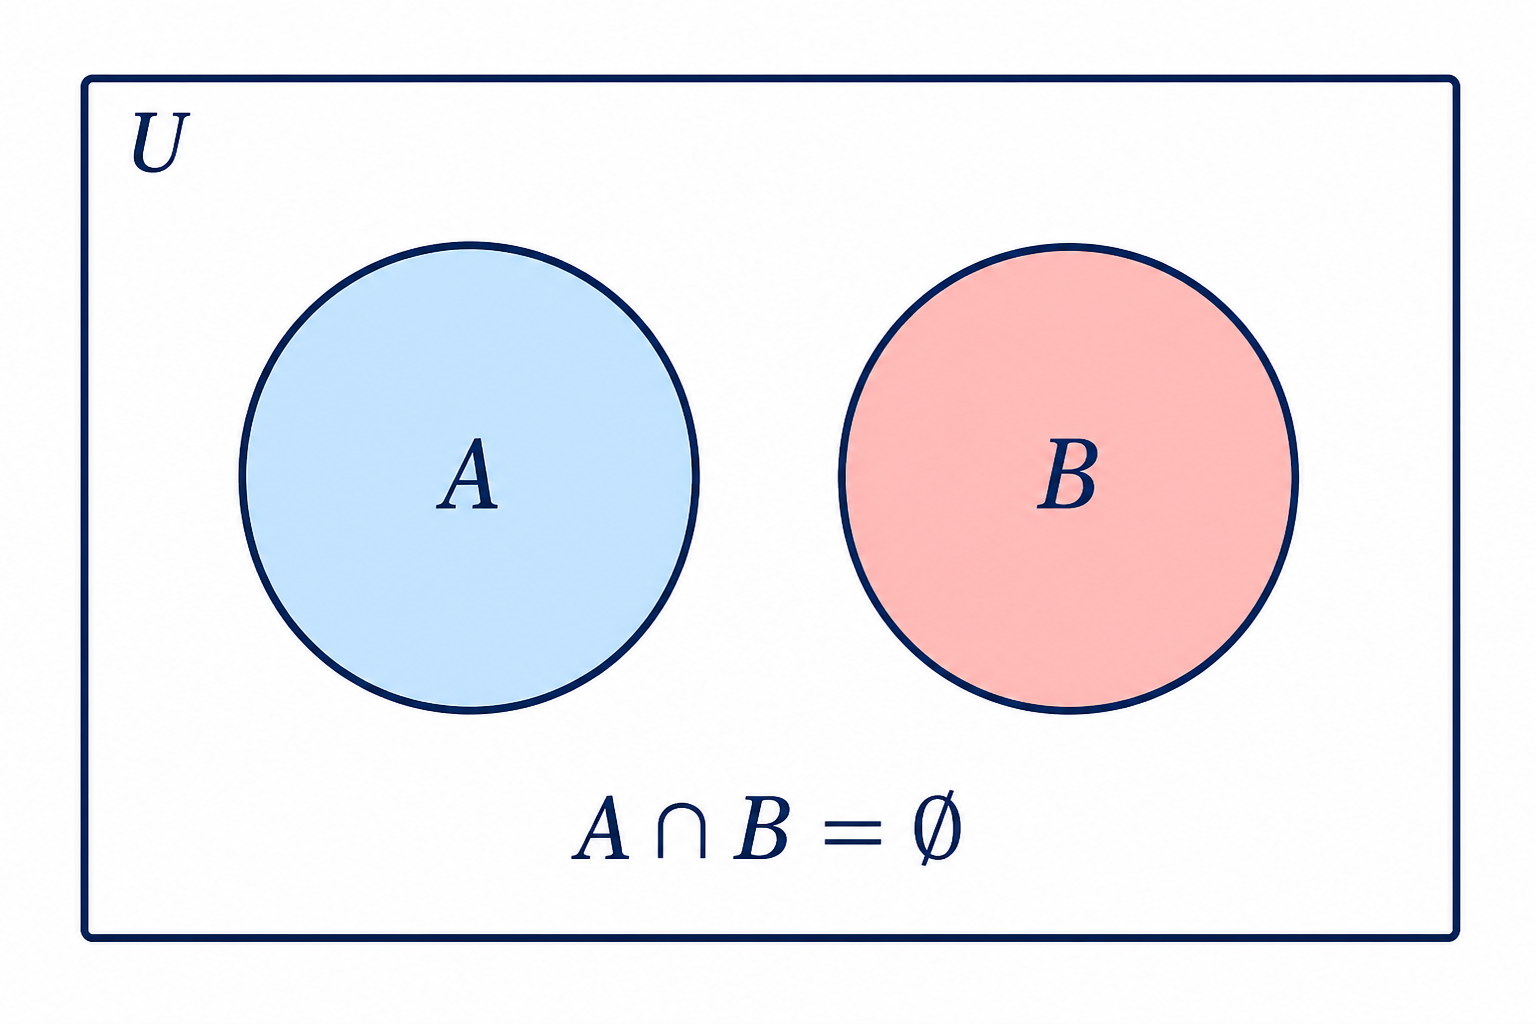
\includegraphics[width=0.62\textwidth]{Figures/png_ready/12-venn-disjoint-generated.png}
    \caption{แผนภาพแสดงเซตไม่มีสมาชิกร่วม เมื่อ $A\cap B=\emptyset$}
    \label{fig:venn-disjoint}
\end{figure}

กรณีพิเศษที่ควรสังเกตคือเมื่ออินเตอร์เซกชันเป็นเซตว่าง ดังรูปที่~\ref{fig:venn-disjoint} ซึ่งวงกลมสองวงไม่มีพื้นที่ทับซ้อนกันเลย เรียกเซตคู่นั้นว่าเซตไม่มีสมาชิกร่วม กรณีนี้ต่างจากรูปที่~\ref{fig:venn-intersection} ที่วงกลมทั้งสองมีพื้นที่ร่วมกัน ในทางปฏิบัติของงานข้อมูล เซตไม่มีสมาชิกร่วมหมายถึงเงื่อนไขสองข้อที่ไม่มีทางเป็นจริงพร้อมกัน เช่น รายการที่มีสถานะยกเลิกกับรายการที่มีสถานะชำระเงินแล้ว

\begin{ex}[การหาอินเตอร์เซกชันของเซต]
กำหนดให้ $A = \{2, 4, 6, 8, 10\}$ และ $B = \{3, 6, 9, 12\}$ จงหา $A \cap B$
\end{ex}

\begin{solution}
หาสมาชิกที่อยู่ทั้งใน $A$ และ $B$ พร้อมกัน
\begin{align*}
A \cap B &= \{2,4,6,8,10\} \cap \{3,6,9,12\}\\
         &= \{6\}
\end{align*}
มีเพียง 6 ที่อยู่ทั้งสองเซต สมาชิกตัวอื่นไม่เป็นสมาชิกร่วม (ถ้า $A \cap B = \emptyset$ จะเรียกว่าเซตไม่มีสมาชิกร่วม)
\label{ex:intersection-step-by-step}
\solhere
\end{solution}

\begin{figure}[H]
    \centering
    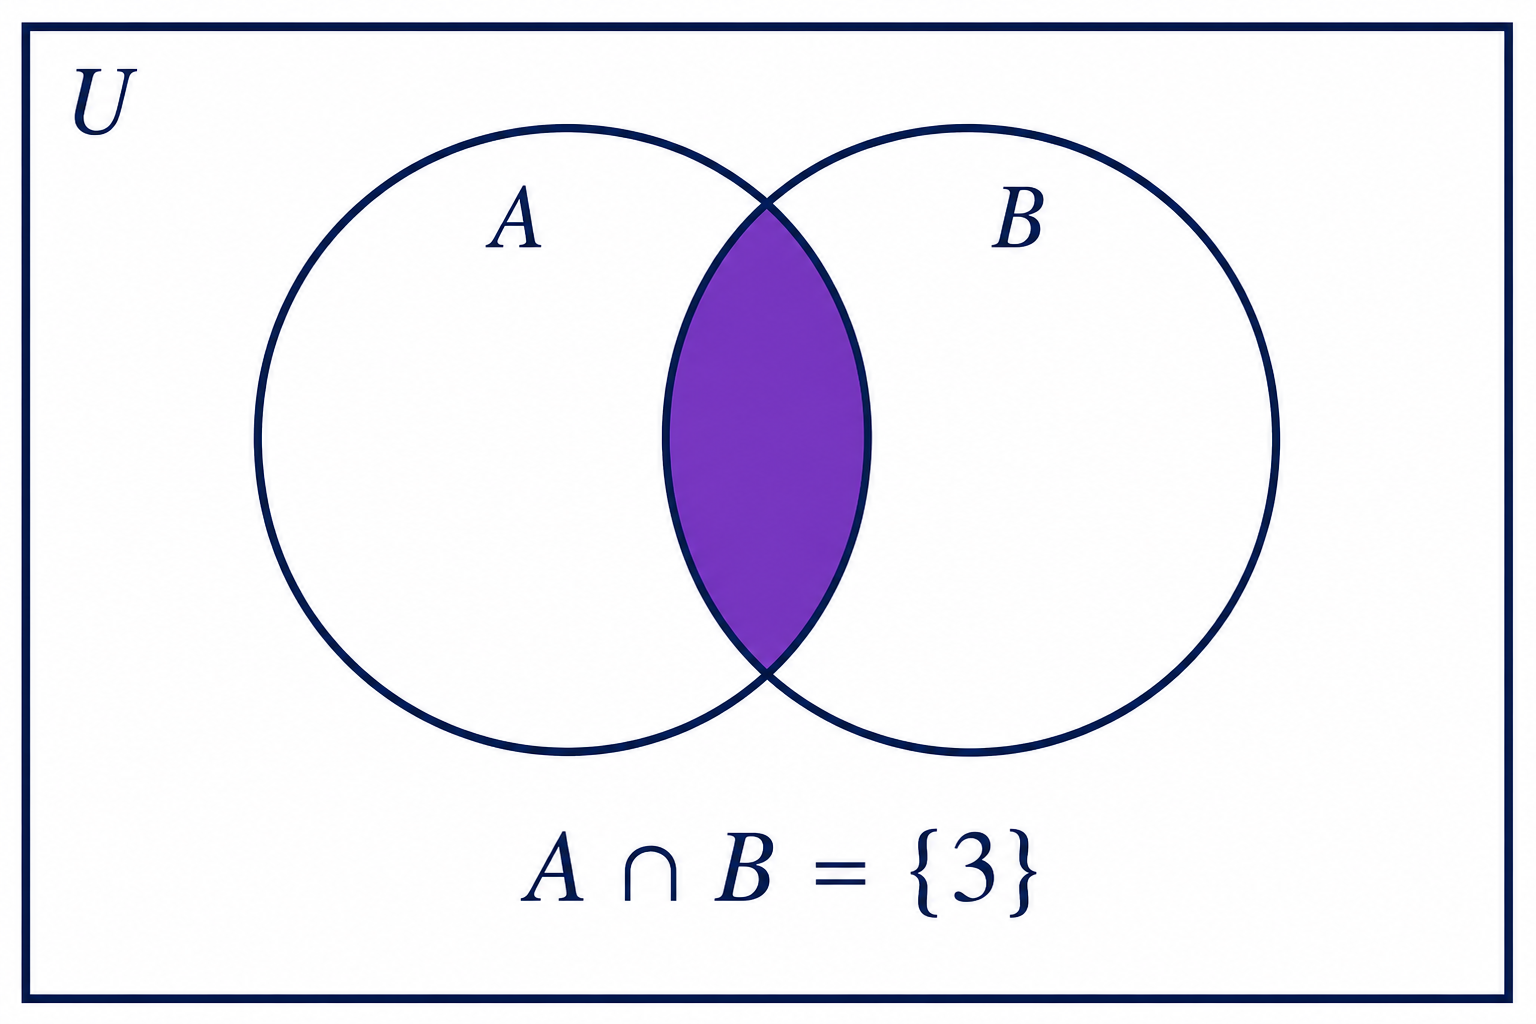
\includegraphics[width=0.65\textwidth]{Figures/png_ready/11-venn-intersection-generated.png}
    \caption{แผนภาพเวนน์แสดงการดำเนินการอินเตอร์เซกชัน $A \cap B$}
    \label{fig:venn-intersection}
\end{figure}

รูปที่ \ref{fig:venn-intersection} แสดงอินเตอร์เซกชัน $A \cap B$ โดยพื้นที่ที่แรเงาคือส่วนที่ทับซ้อนกันของเซต $A$ และเซต $B$ ซึ่งเป็นสมาชิกที่อยู่ทั้งสองเซต


\subsection{ผลต่าง (Set Difference)}
ผลต่างของเซตคือการนำสมาชิกของอีกเซตหนึ่งออกไป เหลือไว้เฉพาะสมาชิกที่อยู่ในเซตแรกแต่ไม่อยู่ในเซตที่สอง การดำเนินการนี้ไม่มีสมบัติสลับที่ กล่าวคือ $A - B$ กับ $B - A$ โดยทั่วไปให้ผลต่างกัน ต่างจากยูเนียนและอินเตอร์เซกชันที่สลับที่ได้ ในทางปฏิบัติผลต่างใช้แทนการคัดกรองข้อมูลออก เช่น การหารายชื่อผู้ที่ลงทะเบียนแล้วแต่ยังไม่ชำระเงิน~\cite{epp2019discrete}

\begin{definition}[ผลต่างระหว่างเซต]
\index{ผลต่างระหว่างเซต!นิยาม}
ผลต่าง ของเซต $A$ และ $B$ เขียนแทนด้วย $A - B$ คือเซตที่ประกอบด้วยสมาชิกที่อยู่ใน $A$ แต่ไม่อยู่ใน $B$ นั่นคือ
\[ A - B = \{x \mid x \in A \text{ และ } x \notin B\} \]
\label{def:set-difference}
\end{definition}

ในทางตรรกศาสตร์ผลต่างสอดคล้องกับ ``$A$ และไม่ $B$'' และโดยทั่วไป $A - B \neq B - A$ กล่าวคือผลต่างไม่มีสมบัติสลับที่ ตัวอย่างเช่น $\{1, 2\} - \{2, 3\} = \{1\}$ ในขณะที่ $\{2, 3\} - \{1, 2\} = \{3\}$

\begin{ex}[การหาผลต่างของเซต]
จงหาผลต่างของเซตต่อไปนี้
\begin{enumerate}
    \item $\{1, 2, 3\} - \{2, 4\}$
    \item $\mathbb{Z} - \mathbb{N}$
    \item $\{1, 2\} - \{1, 2\}$
    \item $\{1, 2\} - \{3, 4\}$
\end{enumerate}
\end{ex}
\begin{solution}
\begin{align*}
\{1,2,3\} - \{2,4\} &= \{1,3\} \quad (\text{นำ 2 ออก; 4 ไม่อยู่ในเซตแรก})\\
\mathbb{Z} - \mathbb{N} &= \{x \in \mathbb{Z} \mid x < 0\} = \mathbb{Z}^-\\
\{1,2\} - \{1,2\} &= \emptyset\\
\{1,2\} - \{3,4\} &= \{1,2\}
\end{align*}
\solhere
\end{solution}

\begin{rem}
ตัวอย่างการนำไปใช้ ให้ $U$ เป็นเซตของนักศึกษาทั้งหมด และ $A$ เป็นเซตของนักศึกษาที่สอบผ่าน แล้ว $U - A$ คือเซตของนักศึกษาที่สอบตก
\end{rem}

\begin{ex}[การหาผลต่างของเซต]
กำหนดให้ $A = \{a, b, c, d, e\}$ และ $B = \{b, d, f\}$ จงหา $A - B$
\end{ex}

\begin{solution}
หาสมาชิกที่อยู่ใน $A$ แต่ไม่อยู่ใน $B$
\begin{align*}
A - B &= \{a,b,c,d,e\} - \{b,d,f\}\\
      &= \{a,c,e\}
\end{align*}
$b$ และ $d$ ถูกนำออกเพราะอยู่ใน $B$; $f$ ไม่อยู่ใน $A$ จึงไม่กระทบผลลัพธ์ (โดยทั่วไป $A - B \neq B - A$)
\label{ex:difference-step-by-step}
\solhere
\end{solution}

\begin{figure}[H]
    \centering
    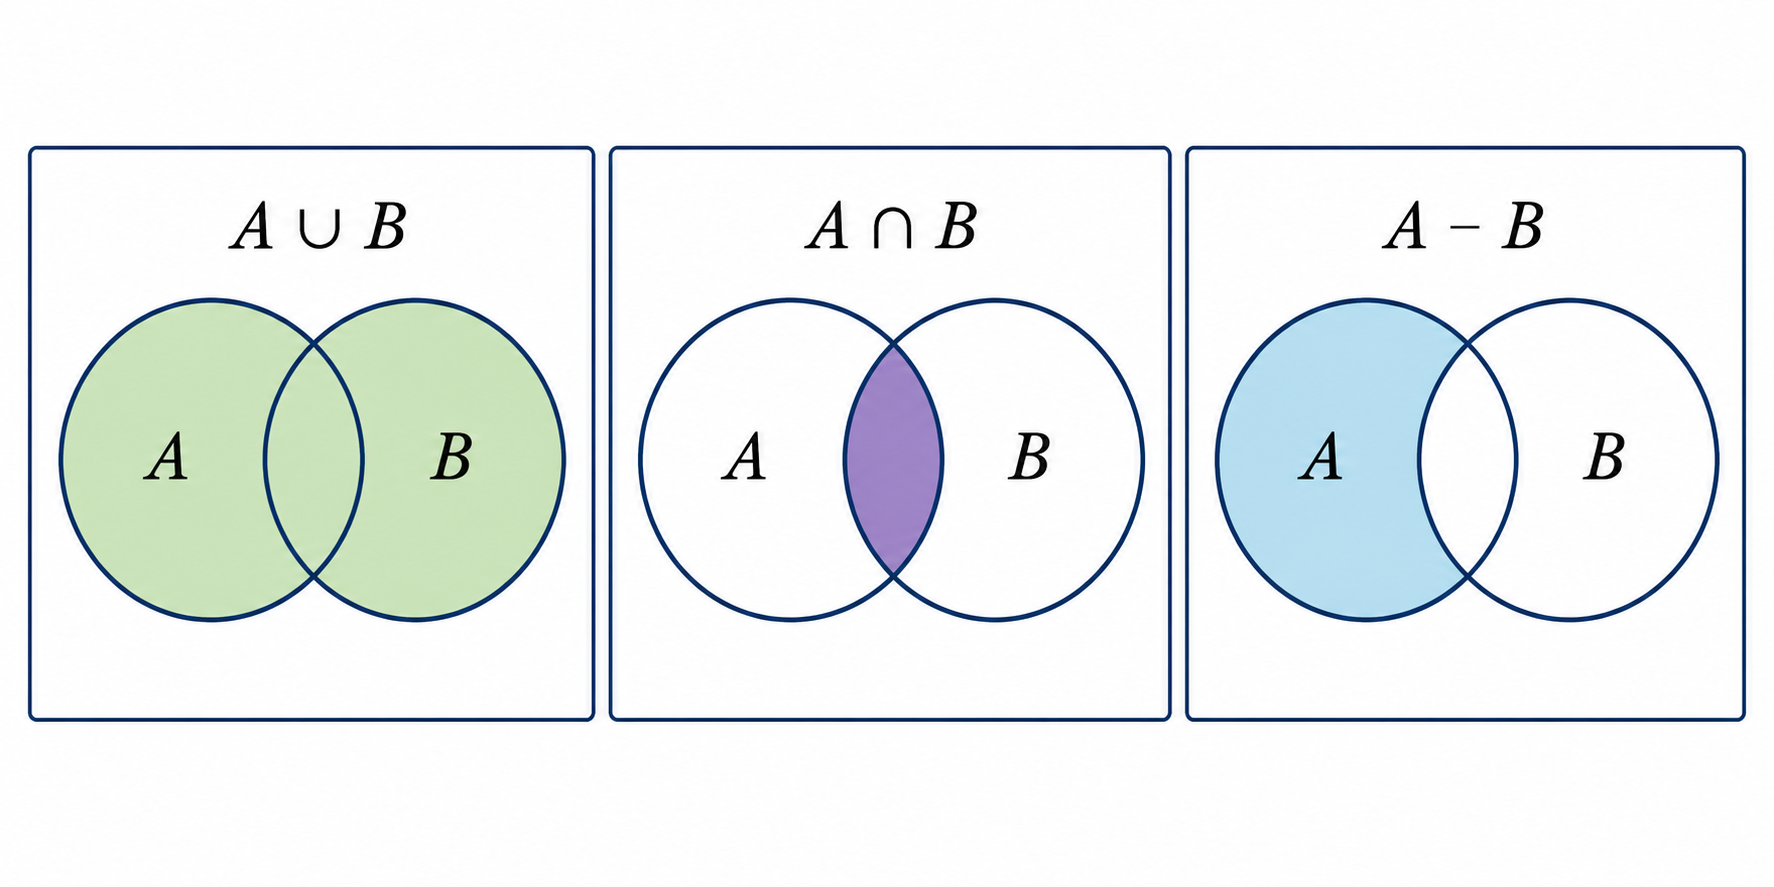
\includegraphics[width=0.90\textwidth]{Figures/png_ready/set-operations-generated.png}
    \caption{การแรเงาพื้นที่ของยูเนียน อินเตอร์เซกชัน และผลต่างของเซต}
    \label{fig:set-difference}
\end{figure}

รูปที่ \ref{fig:set-difference} เปรียบเทียบการแรเงาพื้นที่ของการดำเนินการหลักสามชนิด โดยแผนภาพด้านขวาสุดแสดงผลต่าง $A-B$ ซึ่งเลือกเฉพาะส่วนที่อยู่ใน $A$ แต่ไม่อยู่ใน $B$

\subsection{คอมพลีเมนต์ (Complement)}
คอมพลีเมนต์เป็นการดำเนินการที่ให้ ``สิ่งที่ไม่อยู่ใน $A$'' โดยอ้างอิงกับเอกภพสัมพัทธ์ $U$ สิ่งสำคัญคือต้องกำหนดเอกภพสัมพัทธ์ก่อนเสมอ เพราะคอมพลีเมนต์ขึ้นอยู่กับบริบท เซตเดียวกันจึงมีคอมพลีเมนต์ต่างกันเมื่อเปลี่ยนเอกภพสัมพัทธ์ ตัวอย่างเช่น คอมพลีเมนต์ของเซตจำนวนคู่เมื่อเอกภพสัมพัทธ์เป็นจำนวนเต็ม คือเซตจำนวนคี่ แต่เมื่อเอกภพสัมพัทธ์เป็นจำนวนจริง คอมพลีเมนต์จะรวมจำนวนที่ไม่ใช่จำนวนเต็มเข้าไปด้วย~\cite{johnsonbaugh2016discrete}

\begin{definition}[คอมพลีเมนต์]
\index{คอมพลีเมนต์!นิยาม}
คอมพลีเมนต์ ของเซต $A$ เขียนแทนด้วย $A^c$ หรือ $\overline{A}$ คือเซตที่ประกอบด้วยสมาชิกทั้งหมดในเอกภพสัมพัทธ์ $U$ ที่ไม่อยู่ใน $A$ นั่นคือ
\[ A^c = \{x \in U \mid x \notin A\} = U - A \]
\label{def:complement}
\end{definition}

คอมพลีเมนต์มีสมบัติสำคัญดังนี้
\begin{enumerate}
    \item $A \cup A^c = U$ (กฎคอมพลีเมนต์)
    \item $A \cap A^c = \emptyset$ (กฎการไม่ขัดแย้ง)
    \item $(A^c)^c = A$ (กฎคอมพลีเมนต์ซ้อน)
    \item $A - B = A \cap B^c$ (ผลต่างในรูปอินเตอร์เซกชันกับคอมพลีเมนต์)
\end{enumerate}
สมบัติข้อสุดท้ายมีประโยชน์มาก เพราะช่วยเปลี่ยนผลต่างให้อยู่ในรูปอินเตอร์เซกชันกับคอมพลีเมนต์ ทำให้นำกฎการแจกแจงมาใช้ต่อได้ พิสูจน์สมบัติข้อนี้ได้โดยไล่ตามนิยามของผลต่างและคอมพลีเมนต์ทีละขั้น
\begin{align*}
x \in A - B
&\Leftrightarrow x \in A \ \land\ x \notin B \quad (\text{นิยามของผลต่าง})\\
&\Leftrightarrow x \in A \ \land\ x \in B^c \quad (\text{นิยามของคอมพลีเมนต์})\\
&\Leftrightarrow x \in A \cap B^c \quad (\text{นิยามของอินเตอร์เซกชัน})
\end{align*}
จึงได้ว่า $A - B = A \cap B^c$ สำหรับทุกเซต $A$ และ $B$ ในเอกภพสัมพัทธ์เดียวกัน

ประเด็นที่ผู้เรียนมักมองข้ามคือคอมพลีเมนต์ไม่ได้ขึ้นกับเซต $A$ เพียงอย่างเดียว แต่ขึ้นกับเอกภพสัมพัทธ์ที่เลือกด้วย ตัวอย่างต่อไปนี้แสดงให้เห็นว่าเซต $A$ ชุดเดิมให้คอมพลีเมนต์คนละคำตอบเมื่อเปลี่ยนเอกภพสัมพัทธ์

\begin{ex}[ผลของการเปลี่ยนเอกภพสัมพัทธ์ต่อคอมพลีเมนต์]
กำหนดให้ $A = \{1, 2\}$ จงหา $A^c$ เมื่อกำหนดเอกภพสัมพัทธ์เป็น
\begin{enumerate}
    \item $U_1 = \{1, 2, 3, 4, 5\}$
    \item $U_2 = \{1, 2, 3, 4, 5, 6, 7\}$
\end{enumerate}
\end{ex}
\begin{solution}
คอมพลีเมนต์คือสมาชิกทั้งหมดในเอกภพสัมพัทธ์ที่ไม่อยู่ใน $A$ จึงคำนวณจาก $U - A$ ในแต่ละกรณี
\begin{align*}
A^c &= U_1 - A = \{1,2,3,4,5\} - \{1,2\} = \{3,4,5\}\\
A^c &= U_2 - A = \{1,2,3,4,5,6,7\} - \{1,2\} = \{3,4,5,6,7\}
\end{align*}
เซต $A$ เป็นชุดเดิมทั้งสองกรณี แต่คอมพลีเมนต์ต่างกันเพราะเอกภพสัมพัทธ์ต่างกัน ด้วยเหตุนี้การเขียน $A^c$ โดยไม่ระบุเอกภพสัมพัทธ์จึงไม่มีความหมายที่ชัดเจน ในทางปฏิบัติของงานข้อมูล เอกภพสัมพัทธ์คือขอบเขตของชุดข้อมูลที่กำลังพิจารณา การเปลี่ยนขอบเขตจากทั้งตารางเป็นเฉพาะแถวที่ผ่านการกรองย่อมเปลี่ยนผลของการหาส่วนที่เหลือไปด้วย \solhere
\end{solution}

\begin{ex}[การหาคอมพลีเมนต์ของเซต]
กำหนดให้ $U = \{1, 2, 3, 4, 5, 6, 7, 8\}$ และ $A = \{2, 4, 6, 8\}$ จงหา $A^c$
\end{ex}

\begin{solution}
หาสมาชิกใน $U$ ที่ไม่อยู่ใน $A$
\begin{align*}
A^c &= U - A = \{1,2,3,4,5,6,7,8\} - \{2,4,6,8\}\\
    &= \{1,3,5,7\}
\end{align*}
จำนวนคู่ทั้งหมดอยู่ใน $A$ จึงไม่อยู่ใน $A^c$; จำนวนคี่ทั้งหมดอยู่ใน $A^c$ และตรวจได้ว่า $A \cup A^c = U$
\label{ex:complement-step-by-step}
\solhere
\end{solution}

\begin{figure}[H]
    \centering
    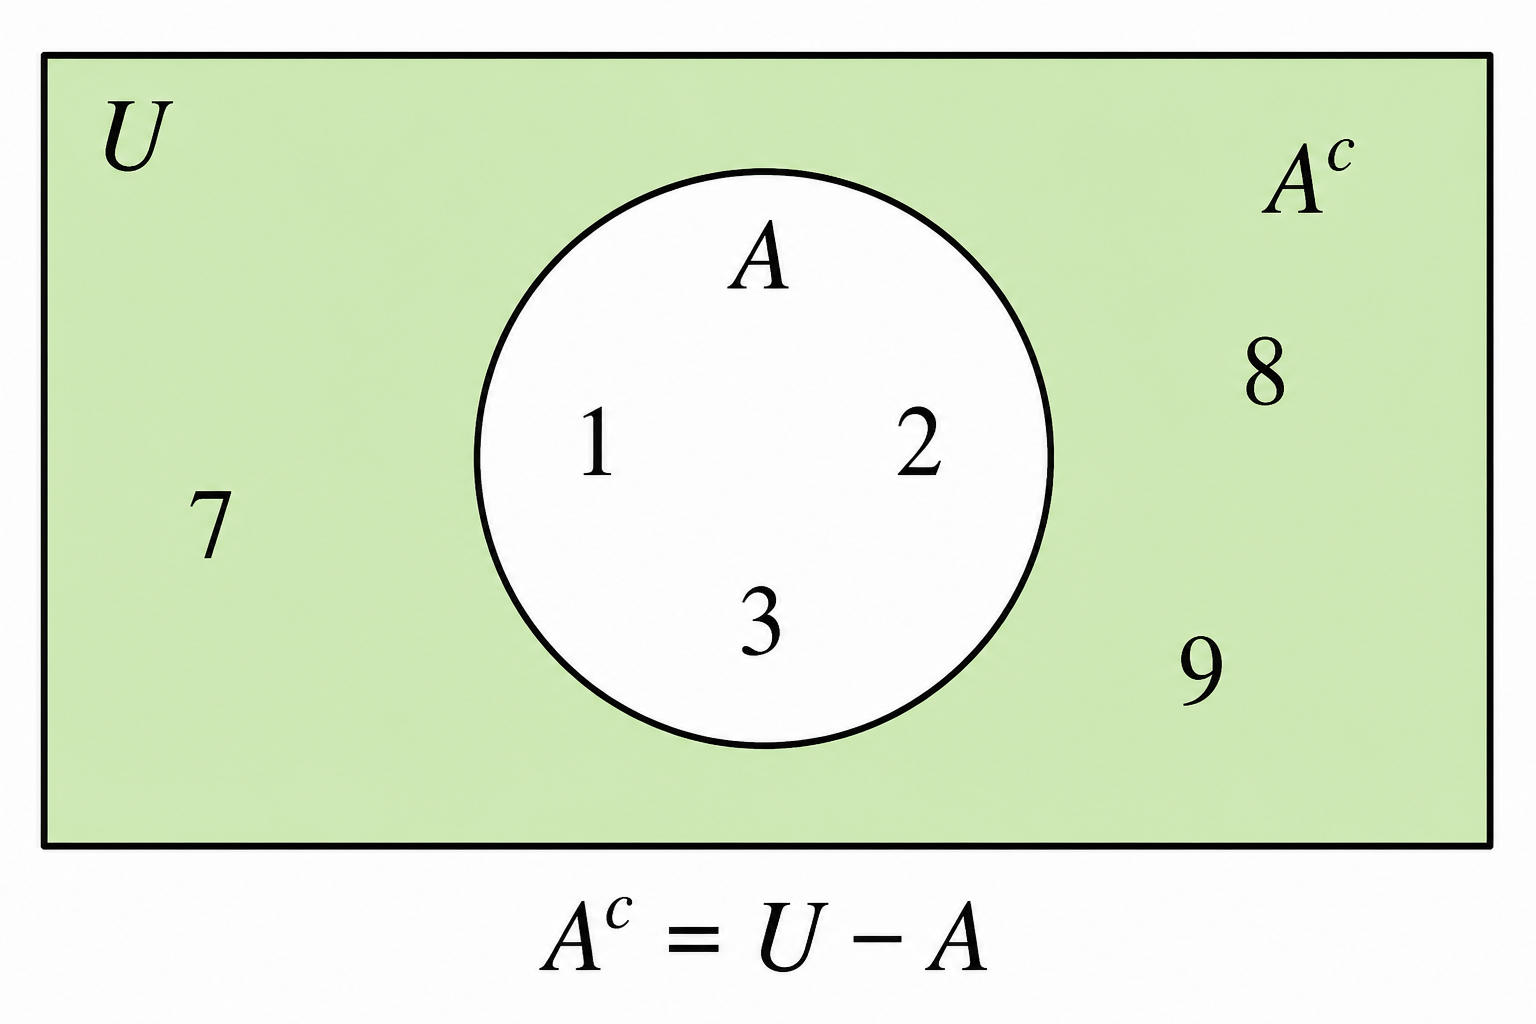
\includegraphics[width=0.65\textwidth]{Figures/png_ready/14-venn-complement-generated.png}
    \caption{แผนภาพเวนน์แสดงคอมพลีเมนต์ $A^c$ ของเซต $A$}
    \label{fig:venn-complement}
\end{figure}

รูปที่ \ref{fig:venn-complement} แสดงคอมพลีเมนต์ $A^c$ ซึ่งคือพื้นที่ทั้งหมดในเอกภพสัมพัทธ์ $U$ ที่ไม่อยู่ในเซต $A$ พื้นที่ที่แรเงาคือ $A^c$

เมื่อศึกษาการดำเนินการครบทั้งสี่ชนิดแล้ว จะพบว่าการดำเนินการเหล่านี้ไม่ได้เป็นอิสระต่อกัน แต่มีสมบัติร่วมกันเป็นชุดที่ใช้จัดรูปนิพจน์ของเซตได้ เช่นเดียวกับที่การบวกและการคูณของจำนวนจริงมีสมบัติการสลับที่และการเปลี่ยนหมู่ สมบัติชุดนี้เรียกรวมว่ากฎพีชคณิตของเซต และเป็นกฎชุดเดียวกับกฎพีชคณิตของประพจน์ใน\autoref{ch:logic} โดยเปลี่ยนจากตัวเชื่อมทางตรรกศาสตร์มาเป็นการดำเนินการระหว่างเซต

\begin{law}[กฎพีชคณิตของการดำเนินการกับเซต (Algebraic Laws for Set Operations)]
สำหรับเซต $A, B, C$ ใดๆ ในเอกภพสัมพัทธ์ $U$ การดำเนินการระหว่างเซตมีสมบัติดังต่อไปนี้

\begin{enumerate}
    \item กฎนิจพล (Idempotent Laws) $A \cup A = A$ และ $A \cap A = A$
    \item กฎเอกลักษณ์ (Identity Laws) $A \cup \emptyset = A$ และ $A \cap U = A$
    \item กฎครอบงำ (Domination Laws) $A \cup U = U$ และ $A \cap \emptyset = \emptyset$
    \item กฎการสลับที่ (Commutative Laws) $A \cup B = B \cup A$ และ $A \cap B = B \cap A$
    \item กฎการเปลี่ยนหมู่ (Associative Laws) $(A \cup B) \cup C = A \cup (B \cup C)$ และ $(A \cap B) \cap C = A \cap (B \cap C)$
    \item กฎการแจกแจง (Distributive Laws) $A \cap (B \cup C) = (A \cap B) \cup (A \cap C)$ และ $A \cup (B \cap C) = (A \cup B) \cap (A \cup C)$
    \item กฎการดูดกลืน (Absorption Laws) $A \cup (A \cap B) = A$ และ $A \cap (A \cup B) = A$
    \item กฎคอมพลีเมนต์ (Complement Laws) $A \cup A^c = U$, $A \cap A^c = \emptyset$, $(A^c)^c = A$, $\emptyset^c = U$, และ $U^c = \emptyset$
\end{enumerate}
\label{thrm:set-algebraic-laws}
\end{law}

\begin{ex}[การพิสูจน์กฎการดูดกลืน]
จงพิสูจน์กฎการดูดกลืน $A \cup (A \cap B) = A$ โดยใช้การพิสูจน์แบบสมาชิก
\label{ex:absorption-proof}
\end{ex}
\begin{solution}
พิสูจน์แบบสมาชิก
\begin{align*}
x \in A \cup (A \cap B)
&\Leftrightarrow x \in A \ \lor\ (x \in A \land x \in B)\\
&\Leftrightarrow x \in A \quad (\text{กฎการดูดกลืนของตรรกศาสตร์})
\end{align*}
$\therefore A \cup (A \cap B) = A$ \solhere
\end{solution}

\begin{figure}[H]
    \centering
    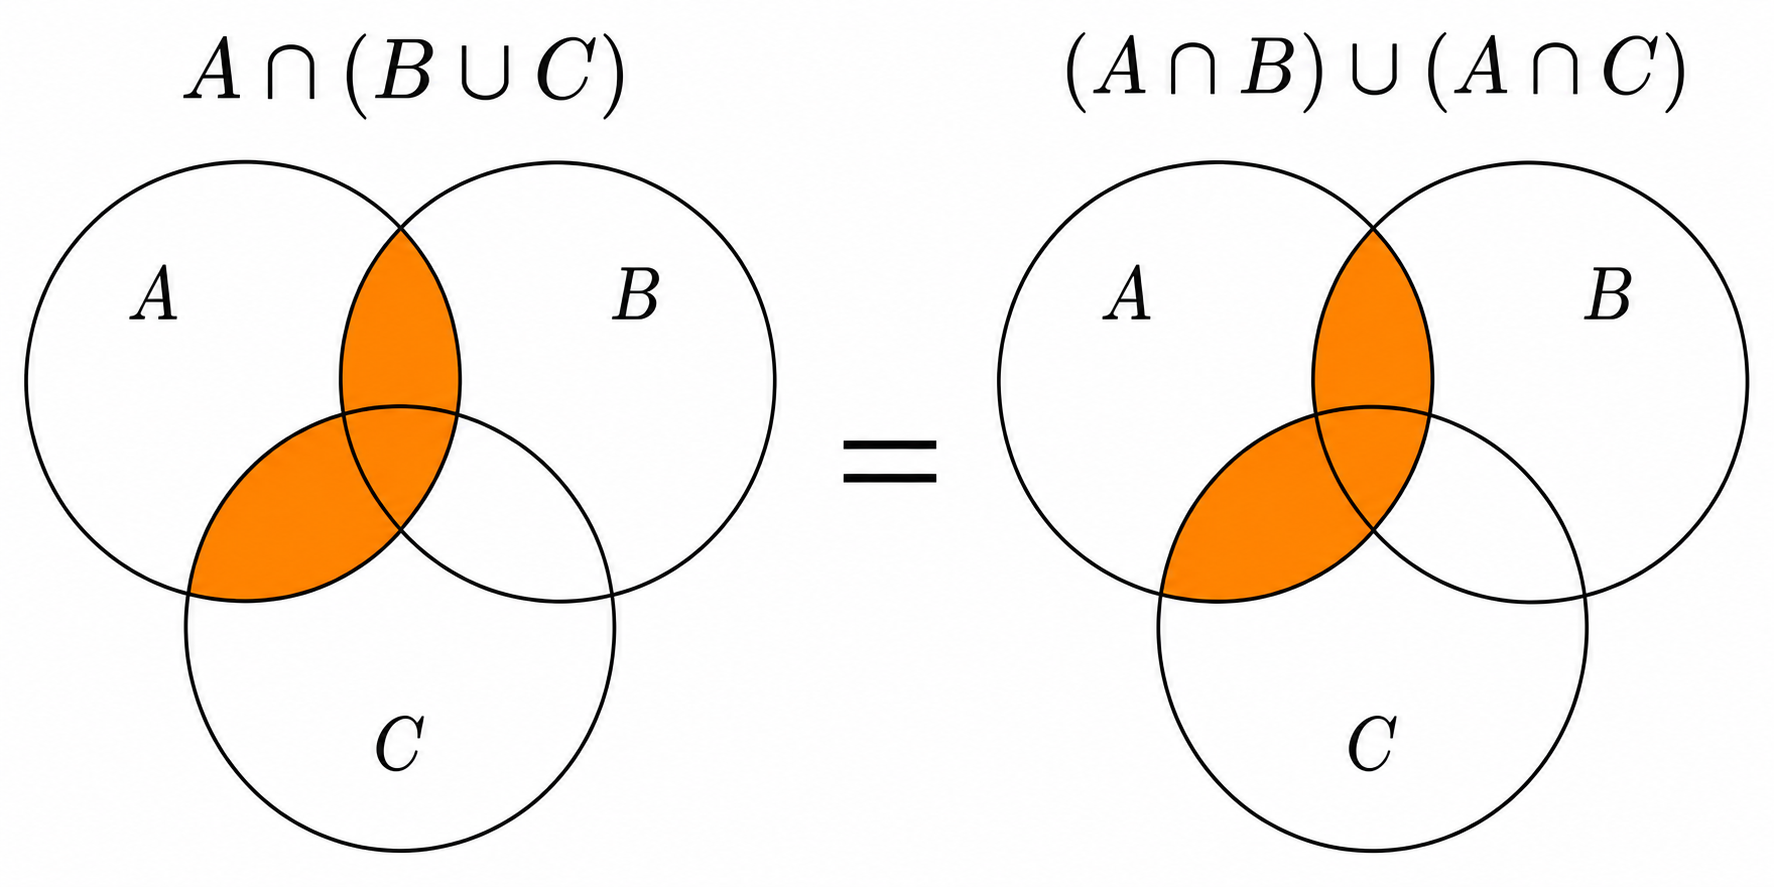
\includegraphics[width=0.65\textwidth]{Figures/png_ready/16-distributive-law-sets-generated.png}
    \caption{แผนภาพเวนน์แสดงกฎการแจกแจง $A \cap (B \cup C) = (A \cap B) \cup (A \cap C)$}
    \label{fig:distributive-law-sets}
\end{figure}

รูปที่ \ref{fig:distributive-law-sets} แสดงกฎการกระจายของเซต โดยฝั่งซ้ายแสดง $A \cap (B \cup C)$ และฝั่งขวาแสดง $(A \cap B) \cup (A \cap C)$ ทั้งสองให้ผลลัพธ์เดียวกัน

\section{กฎเดอมอร์แกน (De Morgan's Laws)}

กฎเดอมอร์แกนตั้งชื่อตามออกัสตัส เดอมอร์แกน (Augustus De Morgan, 1806--1871) นักคณิตศาสตร์ชาวอังกฤษ กฎนี้ระบุความสัมพันธ์ระหว่างคอมพลีเมนต์ ยูเนียน และอินเตอร์เซกชัน ใช้ในการพิสูจน์ทางคณิตศาสตร์และการแปลงนิพจน์ของวงจรดิจิทัล~\cite{halmos1974naive}

\begin{thrm}[กฎเดอมอร์แกนสำหรับเซต]
สำหรับทุกเซต $A$ และ $B$ จะได้ว่า
\begin{enumerate}
    \item $(A \cup B)^c = A^c \cap B^c$ นั่นคือคอมพลีเมนต์ของยูเนียนเท่ากับอินเตอร์เซกชันของคอมพลีเมนต์
    \item $(A \cap B)^c = A^c \cup B^c$ นั่นคือคอมพลีเมนต์ของอินเตอร์เซกชันเท่ากับยูเนียนของคอมพลีเมนต์
\end{enumerate}
\end{thrm}

อ่านกฎทั้งสองข้อเป็นภาษาพูดได้ว่า ข้อแรกคือ ``ไม่อยู่ใน $A$ หรือ $B$'' มีความหมายเดียวกับ ``ไม่อยู่ใน $A$ และไม่อยู่ใน $B$'' ส่วนข้อที่สองคือ ``ไม่อยู่ในทั้ง $A$ และ $B$ พร้อมกัน'' มีความหมายเดียวกับ ``ไม่อยู่ใน $A$ หรือไม่อยู่ใน $B$'' ข้อสังเกตสำคัญคือเมื่อกระจายคอมพลีเมนต์เข้าไปข้างใน ตัวดำเนินการจะสลับชนิดเสมอ ยูเนียนกลายเป็นอินเตอร์เซกชัน และอินเตอร์เซกชันกลายเป็นยูเนียน

\begin{rem}
สังเกตความสอดคล้องกับกฎเดอมอร์แกนในตรรกศาสตร์

\begin{enumerate}
    \item $\neg(p \land q) \equiv \neg p \lor \neg q$ สอดคล้องกับ $(A \cap B)^c = A^c \cup B^c$
    \item $\neg(p \lor q) \equiv \neg p \land \neg q$ สอดคล้องกับ $(A \cup B)^c = A^c \cap B^c$
\end{enumerate}
นี่เป็นตัวอย่างที่แสดงความเชื่อมโยงระหว่างตรรกศาสตร์และทฤษฎีเซต ทั้งสองระบบมีโครงสร้างทางคณิตศาสตร์ที่เหมือนกัน
\end{rem}

\begin{figure}[H]
    \centering
    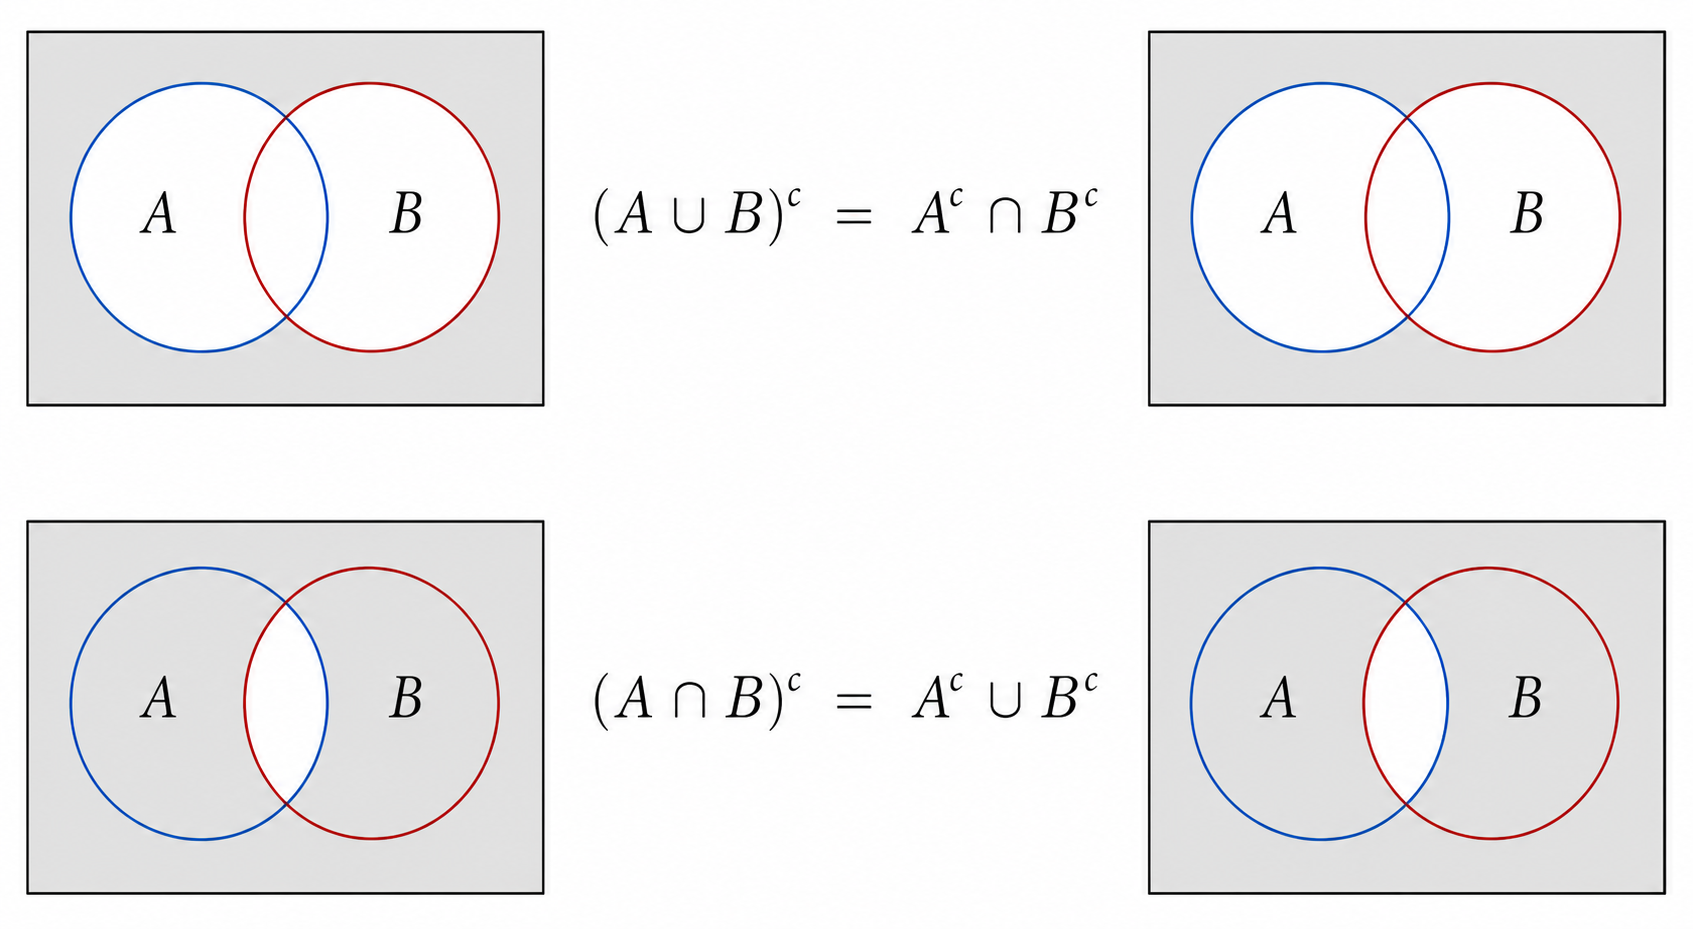
\includegraphics[width=0.65\textwidth]{Figures/png_ready/15-de-morgan-laws-generated.png}
    \caption{แผนภาพเวนน์แสดงกฎเดอมอร์แกน $(A \cup B)^c = A^c \cap B^c$ และ $(A \cap B)^c = A^c \cup B^c$}
    \label{fig:de-morgan-laws}
\end{figure}

รูปที่ \ref{fig:de-morgan-laws} แสดงกฎเดอมอร์แกนทั้งสองข้อ โดยฝั่งบนแสดงว่าคอมพลีเมนต์ของยูเนียนเท่ากับอินเตอร์เซกชันของคอมพลีเมนต์ และฝั่งล่างแสดงว่าคอมพลีเมนต์ของอินเตอร์เซกชันเท่ากับยูเนียนของคอมพลีเมนต์

กฎเดอมอร์แกนถูกนำไปใช้มากในการออกแบบวงจรดิจิทัล เพราะบางครั้งวงจรที่ออกแบบไว้ใช้ประตูตรรกะชนิดหนึ่ง แต่ชิ้นส่วนที่มีอยู่จริงเป็นอีกชนิดหนึ่ง กฎนี้ระบุวิธีแปลงประตูตรรกะแบบและให้เป็นประตูตรรกะแบบหรือโดยเพิ่มการนิเสธที่ขาเข้าและขาออก และแปลงย้อนกลับได้เช่นกัน โดยผลลัพธ์ของวงจรไม่เปลี่ยน รายละเอียดของการแปลงอยู่ใน\autoref{ch:boolean}

\begin{ex}[การพิสูจน์กฎเดอมอร์แกนข้อที่หนึ่ง]
พิสูจน์ $(A \cup B)^c = A^c \cap B^c$
\end{ex}
\begin{solution}
พิสูจน์แบบสมาชิก
\begin{align*}
x \in (A \cup B)^c
&\Leftrightarrow x \notin A \cup B\\
&\Leftrightarrow \neg(x \in A \lor x \in B)\\
&\Leftrightarrow \neg(x \in A) \land \neg(x \in B) \quad (\text{กฎเดอมอร์แกนของตรรกศาสตร์})\\
&\Leftrightarrow x \in A^c \land x \in B^c\\
&\Leftrightarrow x \in A^c \cap B^c
\end{align*}
$\therefore (A \cup B)^c = A^c \cap B^c$ \solhere
\end{solution}

\section{เพาเวอร์เซต (Power Set)}
บางครั้งเราไม่ได้สนใจเพียงสมาชิกของเซต แต่สนใจ ``เซตย่อยทั้งหมด'' ที่สร้างจากเซตนั้นได้ การรวบรวมเซตย่อยทุกแบบเข้าด้วยกันเป็นเซตใหม่ นำไปสู่แนวคิดเพาเวอร์เซต ประเด็นที่ต้องระวังคือสมาชิกของเพาเวอร์เซตเป็นเซต ไม่ใช่สมาชิกของเซตเดิม และเพาเวอร์เซตของเซตที่มีสมาชิก $n$ ตัวมีสมาชิกทั้งหมด $2^n$ ตัว ซึ่งเติบโตเร็วมากเมื่อ $n$ เพิ่มขึ้น~\cite{enderton1977settheory}

\begin{definition}[เพาเวอร์เซต]
\index{เพาเวอร์เซต!นิยาม}
เพาเวอร์เซต ของเซต $A$ เขียนแทนด้วย $\mathcal{P}(A)$ หรือ $2^A$ คือเซตที่ประกอบด้วยเซตย่อยทั้งหมดของ $A$ นั่นคือ
\[ \mathcal{P}(A) = \{B \mid B \subseteq A\} \]
\label{def:power-set}
\end{definition}

เพาเวอร์เซตเป็น ``เซตของเซต'' เพราะสมาชิกของมันคือเซตย่อยของ $A$ สมบัติสำคัญคือ ถ้า $|A| = n$ แล้ว $|\mathcal{P}(A)| = 2^n$ เหตุผลคือในการสร้างเซตย่อยหนึ่ง สมาชิกแต่ละตัวของ $A$ มีทางเลือก 2 ทาง คือ ``อยู่'' หรือ ``ไม่อยู่'' ในเซตย่อยนั้น จำนวนเซตย่อยทั้งหมดจึงเท่ากับ $2^n$ ด้วยเหตุนี้สัญลักษณ์ $2^A$ จึงสื่อความหมายได้ตรง เพราะ $|\mathcal{P}(A)| = 2^{|A|}$

\begin{ex}[การหาเพาเวอร์เซต]
จงหาเพาเวอร์เซตของเซตต่อไปนี้
\begin{enumerate}
    \item $\{1, 2\}$
    \item $\emptyset$
    \item $\{a\}$
    \item $\{1, 2, 3\}$
\end{enumerate}
\end{ex}
\begin{solution}
\begin{align*}
\mathcal{P}(\{1,2\}) &= \{\emptyset, \{1\}, \{2\}, \{1,2\}\} \quad (2^2 = 4)\\
\mathcal{P}(\emptyset) &= \{\emptyset\} \quad (2^0 = 1,\ \text{มีสมาชิกคือ } \emptyset)\\
\mathcal{P}(\{a\}) &= \{\emptyset, \{a\}\} \quad (2^1 = 2)\\
\mathcal{P}(\{1,2,3\}) &= \{\emptyset, \{1\}, \{2\}, \{3\}, \{1,2\}, \{1,3\}, \{2,3\}, \{1,2,3\}\} \quad (2^3 = 8)
\end{align*}
\solhere
\end{solution}


\section{ผลคูณคาร์ทีเซียน (Cartesian Product)}
\label{sec:cartesian-product}

การดำเนินการที่ผ่านมาทั้งหมดสร้างเซตใหม่จากสมาชิกชุดเดิม แต่ในการอธิบายความสัมพันธ์ระหว่างข้อมูลสองชุด สิ่งที่ต้องการคือการจับคู่สมาชิกจากเซตหนึ่งเข้ากับสมาชิกจากอีกเซตหนึ่ง เช่น การจับคู่รหัสนักศึกษากับรายวิชาที่ลงทะเบียน การจับคู่เช่นนี้ต้องรักษาลำดับไว้ เพราะคู่ที่ว่า ``นักศึกษา ก ลงทะเบียนวิชา ข'' ไม่เหมือนกับ ``วิชา ก ลงทะเบียนนักศึกษา ข'' หัวข้อนี้จึงเริ่มจากแนวคิดคู่อันดับ แล้วจึงนิยามผลคูณคาร์ทีเซียนซึ่งรวบรวมคู่อันดับที่เป็นไปได้ทั้งหมด แนวคิดนี้เป็นรากฐานโดยตรงของความสัมพันธ์และฟังก์ชันใน\autoref{ch:relations}

คู่อันดับ $(a, b)$ แตกต่างจากเซต $\{a, b\}$ ตรงที่มีลำดับ กล่าวคือ $(a, b) \neq (b, a)$ ยกเว้นกรณี $a = b$ และ $(a, b) = (c, d)$ ก็ต่อเมื่อ $a = c$ และ $b = d$ ชื่อผลคูณคาร์ทีเซียนมาจากชื่อของเรอเน เดการ์ต (Rene Descartes) นักคณิตศาสตร์ผู้พัฒนาเรขาคณิตวิเคราะห์ $\mathbb{R} \times \mathbb{R} = \mathbb{R}^2$ คือระนาบ 2 มิติที่เราใช้กันทั่วไป~\cite{lipschutz1998settheory}

\begin{definition}[ผลคูณคาร์ทีเซียน]
\index{ผลคูณคาร์ทีเซียน!นิยาม}
ผลคูณคาร์ทีเซียน ของเซต $A$ และ $B$ เขียนแทนด้วย $A \times B$ คือเซตของคู่อันดับ $(a, b)$ โดยที่ $a \in A$ และ $b \in B$ นั่นคือ
\[ A \times B = \{(a, b) \mid a \in A \text{ และ } b \in B\} \]
\end{definition}

\begin{ex}[การหาผลคูณคาร์ทีเซียน]
จงหาผลคูณคาร์ทีเซียนต่อไปนี้
\begin{enumerate}
    \item $\{1, 2\} \times \{a, b\}$
    \item $\mathbb{R} \times \mathbb{R}$
    \item $\emptyset \times A$ เมื่อ $A$ เป็นเซตใดๆ
\end{enumerate}
\end{ex}
\begin{solution}
\begin{align*}
\{1,2\} \times \{a,b\} &= \{(1,a),(1,b),(2,a),(2,b)\} \quad (\text{ลำดับสำคัญ เพราะ } (1,a) \neq (a,1))\\
\mathbb{R} \times \mathbb{R} &= \mathbb{R}^2 \quad (\text{ระนาบ 2 มิติ})\\
\emptyset \times A &= A \times \emptyset = \emptyset
\end{align*}
\solhere
\end{solution}

\begin{rem}[ข้อสังเกตเรื่องจำนวนสมาชิกของผลคูณคาร์ทีเซียน]
ถ้า $|A| = m$ และ $|B| = n$ แล้ว $|A \times B| = m \cdot n$ เพราะทุกสมาชิกใน $A$ สามารถจับคู่กับทุกสมาชิกใน $B$ ได้ จึงมี $m \times n$ คู่ และ $\mathbb{R} \times \mathbb{R}$ มี cardinality เท่ากับ $|\mathbb{R}|^2$ ซึ่งเป็น uncountable เช่นเดียวกับ $\mathbb{R}$
\end{rem}

\begin{prop}[สมบัติของผลคูณคาร์ทีเซียน]
ผลคูณคาร์ทีเซียนมีสมบัติดังนี้
\begin{enumerate}
    \item $A \times (B \cup C) = (A \times B) \cup (A \times C)$
    \item $A \times (B \cap C) = (A \times B) \cap (A \times C)$
    \item $(A \cup B) \times C = (A \times C) \cup (B \times C)$
    \item $(A \cap B) \times C = (A \times C) \cap (B \times C)$
\end{enumerate}
สังเกตว่า Cartesian Product กระจายเหนือ union และ intersection ในทางที่คล้ายกับการกระจายการคูณเหนือการบวก
\end{prop}

\section{การนับจำนวนสมาชิกของเซต (Cardinality)}

เมื่อมีเซตหนึ่ง คำถามพื้นฐานที่สุดคือเซตนั้นมีสมาชิกกี่ตัว การนับจำนวนสมาชิกเป็นสิ่งที่เราทำในชีวิตประจำวันอยู่แล้ว เช่น นับจำนวนนักศึกษาในห้องหรือจำนวนสินค้าในตะกร้า ในทางคณิตศาสตร์เรียกจำนวนสมาชิกของเซตว่าคาร์ดินัลลิตี้ สำหรับเซตจำกัดค่านี้เป็นจำนวนเต็มไม่ติดลบธรรมดา แต่สำหรับเซตอนันต์ต้องอาศัยการจับคู่หนึ่งต่อหนึ่งเพื่อเปรียบเทียบขนาด ซึ่งจะศึกษาในหัวข้อท้ายบท~\cite{rosen2019discrete}

\begin{definition}[จำนวนสมาชิกของเซต (Cardinality)]
\index{จำนวนสมาชิกของเซต!นิยาม}
จำนวนสมาชิกของเซต หรือคาร์ดินัลลิตี้ (cardinality) ของเซต $A$ เขียนแทนด้วย $|A|$ คือจำนวนสมาชิกของเซต $A$
\end{definition}

สำหรับเซตจำกัด จำนวนสมาชิกของเซตคือจำนวนที่นับได้โดยตรง เช่น ถ้า $A = \{a, e, i, o, u\}$ แล้ว $|A| = 5$ ส่วนเซตอนันต์ต้องใช้แนวคิดที่ละเอียดกว่านี้ คือการจับคู่สมาชิกแบบหนึ่งต่อหนึ่งระหว่างเซต และในบางกรณีต้องใช้ข้อโต้แย้งแนวทแยงของคันทอร์ (Cantor's diagonal argument) ซึ่งจะกล่าวถึงในหัวข้อเซตนับได้และเซตนับไม่ได้ต่อไป

การนับจำนวนสมาชิกเป็นพื้นฐานของการนับเชิงการจัด (combinatorics) และใช้มากในการนับจำนวนโอกาสทั้งหมดที่เป็นไปได้

\begin{principle}[หลักการรวม-การแยก (Inclusion-Exclusion Principle)]
สำหรับเซตจำกัด $A$ และ $B$ ใด ๆ จะได้ว่า
\begin{enumerate}
    \item $|A \cup B| = |A| + |B| - |A \cap B|$
    \item ถ้า $A$ และ $B$ เป็นเซตไม่มีสมาชิกร่วม คือ $A \cap B = \emptyset$ แล้ว $|A \cup B| = |A| + |B|$
\end{enumerate}
\end{principle}

\begin{figure}[H]
    \centering
    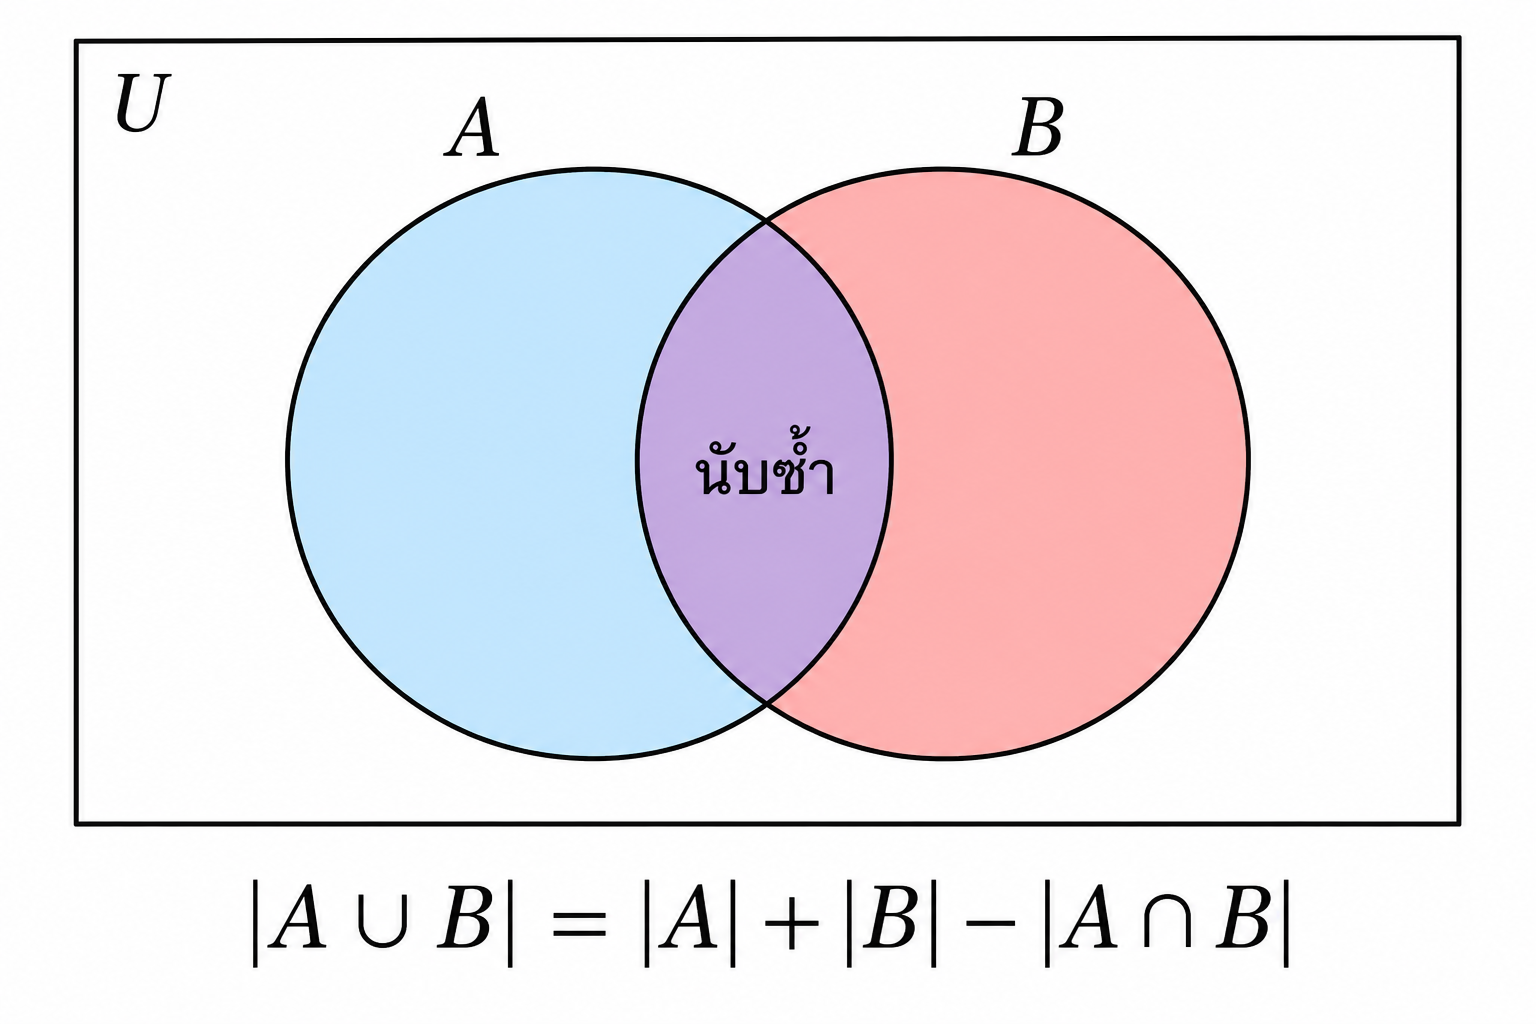
\includegraphics[width=0.70\textwidth]{Figures/png_ready/17-venn-inclusion-exclusion-generated.png}
    \caption{แผนภาพประกอบหลักการรวม-การแยก แสดงการหักส่วนซ้ำ $A\cap B$ ออกจาก $|A|+|B|$}
    \label{fig:venn-inclusion-exclusion}
\end{figure}

หลักการรวม-การแยกใช้เมื่อต้องการนับจำนวนสมาชิกของยูเนียน ถ้านับ $|A| + |B|$ โดยตรง สมาชิกที่อยู่ทั้งสองเซตจะถูกนับซ้ำ จึงต้องลบออก เหตุผลนี้เห็นได้ชัดจากรูปที่~\ref{fig:venn-inclusion-exclusion} ซึ่งพื้นที่ตรงกลางที่วงกลมสองวงซ้อนกันถูกระบายรวมอยู่ทั้งใน $|A|$ และ $|B|$ การบวกสองจำนวนนี้จึงนับพื้นที่ตรงกลางสองครั้ง การลบ $|A \cap B|$ ออกหนึ่งครั้งจึงทำให้ได้จำนวนที่ถูกต้องพอดี

\begin{ex}[การนับสมาชิกของยูเนียนด้วยหลักการเพิ่มเข้าตัดออก]
ถ้า $A = \{1, 2, 3, 4\}$, $B = \{3, 4, 5, 6\}$ จงหา $|A \cup B|$
\end{ex}
\begin{solution}
\begin{align*}
A \cap B &= \{3,4\} \Rightarrow |A \cap B| = 2\\
|A \cup B| &= |A| + |B| - |A \cap B| = 4 + 4 - 2 = 6
\end{align*}
ตรวจคำตอบได้จาก $|\{1,2,3,4,5,6\}| = 6$ ถ้านับ $|A|+|B| = 8$ โดยไม่หักส่วนที่ซ้อนกันออก ผลจะเกินจริง เพราะ 3 และ 4 ถูกนับสองครั้ง \solhere
\end{solution}

การประยุกต์ใช้ในชีวิตจริง ดังนี้

\begin{enumerate}
    \item นักศึกษา 30 คน 15 คนเรียนภาษาอังกฤษ 20 คนเรียนคณิตศาสตร์ มีนักศึกษากี่คนที่เรียนอย่างน้อยหนึ่งวิชา? ถ้าไม่มีนักศึกษาคนใดเรียนทั้งสองวิชา (disjoint) ก็ $15 + 20 = 35$ ซึ่งมากกว่า 30 แสดงว่าต้องมีนักศึกษาที่เรียนทั้งสองวิชา
\end{enumerate}

\begin{thrm}
สำหรับเซต 3 เซต ดังนี้

\[
|A \cup B \cup C| = |A| + |B| + |C| - |A \cap B| - |A \cap C| - |B \cap C| + |A \cap B \cap C|
\]

สูตรนี้ขยายจาก 2 เซต โดยลบ intersection ของทุกคู่ แล้วบวก intersection ของทั้งสามกลับ (เพราะถูกลบเกินไป)
\end{thrm}

\begin{ex}[ตัวอย่างตรวจพบข้อมูลไม่สอดคล้อง]
ในห้องเรียน 20 คน มี 12 คนเรียนคณิตศาสตร์ 15 คนเรียนฟิสิกส์ และ 10 คนเรียนเคมี นอกจากนี้ 6 คนเรียนคณิตศาสตร์และฟิสิกส์ 5 คนเรียนคณิตศาสตร์และเคมี 4 คนเรียนฟิสิกส์และเคมี และ 2 คนเรียนทั้งสามวิชา มีกี่คนที่เรียนอย่างน้อยหนึ่งวิชา?
\end{ex}
\begin{solution}
กำหนด $M$ (คณิตศาสตร์), $P$ (ฟิสิกส์), $C$ (เคมี) โดย $|M|=12$, $|P|=15$, $|C|=10$, $|M \cap P|=6$, $|M \cap C|=5$, $|P \cap C|=4$, $|M \cap P \cap C|=2$
\begin{align*}
|M \cup P \cup C| &= |M|+|P|+|C|-|M\cap P|-|M\cap C|-|P\cap C|+|M\cap P\cap C|\\
                  &= 12+15+10-6-5-4+2 = 24
\end{align*}
แต่ $24 > 20$ (จำนวนนักเรียนทั้งหมด) เป็นไปไม่ได้ แสดงว่าข้อมูลที่ให้มาไม่สอดคล้องกัน ควรย้อนกลับไปตรวจแหล่งข้อมูลก่อนสรุปผล \solhere
\end{solution}

\begin{thrm}[จำนวนสมาชิกของผลคูณคาร์ทีเซียน (Cardinality of Cartesian Product)]
\label{thrm:cardinality-cartesian}
ให้ $A$ และ $B$ เป็นเซตจำกัด (finite sets) ใด ๆ จำนวนสมาชิกของผลคูณคาร์ทีเซียน $A \times B$ จะเท่ากับผลคูณของจำนวนสมาชิกของเซต $A$ และเซต $B$ นั่นคือ
\[
|A \times B| = |A| \cdot |B|
\]
แนวคิดการพิสูจน์มีดังนี้ คู่อันดับ $(a, b) \in A \times B$ เกิดจากการเลือกสมาชิกตัวแรก $a$ จากเซต $A$ ซึ่งมีทางเลือก $|A|$ วิธี และเลือกสมาชิกตัวที่สอง $b$ จากเซต $B$ ซึ่งมีทางเลือก $|B|$ วิธี โดยการเลือกแต่ละตำแหน่งเป็นอิสระต่อกัน ตามหลักการคูณทางการนับ จะได้จำนวนคู่อันดับทั้งหมดเท่ากับ $|A| \cdot |B|$ ตัว
\end{thrm}

\begin{thrm}[จำนวนสมาชิกของเพาเวอร์เซต (Cardinality of Power Set)]
\label{thrm:cardinality-powerset}
ให้ $A$ เป็นเซตจำกัดที่มีสมาชิก $n$ ตัว นั่นคือ $|A| = n$ จำนวนสมาชิกของเพาเวอร์เซต $\mathcal{P}(A)$ (ซึ่งเท่ากับจำนวนสับเซตทั้งหมดของ $A$) จะเท่ากับ $2^n$ นั่นคือ
\[
|\mathcal{P}(A)| = 2^{|A|}
\]
แนวคิดการพิสูจน์มีดังนี้ ในการสร้างสับเซต $S \subseteq A$ สมาชิกแต่ละตัวใน $A$ มีทางเลือก 2 ทางเสมอ คือ ``เลือกให้อยู่ใน $S$'' หรือ ``ไม่เลือกให้อยู่ใน $S$'' เมื่อมีสมาชิกทั้งหมด $n$ ตัว การสร้างสับเซตจึงประกอบด้วยการตัดสินใจ $n$ ครั้งติดต่อกัน ตามหลักการคูณ จะได้จำนวนสับเซตที่เป็นไปได้ทั้งหมดเท่ากับ
\[
\underbrace{2 \times 2 \times \cdots \times 2}_{n \text{ ครั้ง}} = 2^n
\]
นอกจากนี้ ยังสามารถพิสูจน์ด้วยทฤษฎีบททวินาม (binomial theorem) จากการรวมจำนวนสับเซตที่มีขนาด $k$ (เลือกสมาชิก $k$ ตัวจาก $n$ ตัว) สำหรับ $k = 0, 1, \ldots, n$ จะได้
\[
|\mathcal{P}(A)| = \sum_{k=0}^{n} \binom{n}{k} = (1 + 1)^n = 2^n
\]
\end{thrm}

นี่เป็นเหตุผลว่าทำไมเพาเวอร์เซตจึงมีการเติบโตเชิงเลขชี้กำลัง (Exponential Growth) เมื่อ $|A|$ เพิ่มขึ้นเพียง 1 สมาชิก ขนาดของเพาเวอร์เซต $|\mathcal{P}(A)|$ จะเพิ่มขึ้นเป็น 2 เท่าเสมอ

\section{การประยุกต์ในวิทยาการคอมพิวเตอร์}

หัวข้อนี้แสดงการใช้แนวคิดเซตในวิทยาการคอมพิวเตอร์สามด้าน ได้แก่ การแทนเซตด้วยโครงสร้างข้อมูล การสืบค้นข้อมูลในฐานข้อมูล และการจัดเก็บสมาชิกด้วยฟังก์ชันแฮช~\cite{gersting2014structures}

\subsection{การแทนเซตในโครงสร้างข้อมูล}

ในการเขียนโปรแกรม การแทนเซตแต่ละวิธีใช้พื้นที่จัดเก็บและเวลาตรวจสอบสมาชิกต่างกัน การเลือกวิธีขึ้นกับขนาดของเอกภพสัมพัทธ์และการดำเนินการที่ต้องใช้ หัวข้อนี้อธิบายการแทนเซตด้วยเวกเตอร์บิตและตารางแฮช~\cite{gersting2014structures}

\begin{ex}[การแทนด้วยเวกเตอร์บิต (Bit Vector Representation)]
จงแทนเซต $A = \{2, 5, 7\}$ ในเอกภพสัมพัทธ์ $U = \{1, 2, 3, 4, 5, 6, 7, 8, 9\}$ ด้วยเวกเตอร์บิต
\end{ex}
\begin{solution}
กำหนดบิตตามตำแหน่งของสมาชิกใน $U = \{1,2,\ldots,9\}$ โดยให้บิตมีค่า 1 เมื่อสมาชิกอยู่ใน $A = \{2,5,7\}$ และมีค่า 0 เมื่อสมาชิกไม่อยู่ใน $A$
\begin{center}
$U$:\quad \texttt{1 2 3 4 5 6 7 8 9}\\[2pt]
$A$:\quad \texttt{0 1 0 0 1 0 1 0 0}
\end{center}
ได้เวกเตอร์บิต $\texttt{010010100}$ ซึ่งมีค่าเท่ากับ $148_{10}$ เมื่อมองเป็นจำนวนฐานสอง การตรวจสอบสมาชิกทำได้โดยอ่านบิตที่ตำแหน่งนั้น จึงใช้เวลา $O(1)$ การยูเนียน อินเตอร์เซกชัน และคอมพลีเมนต์ดำเนินการแบบบิตต่อบิต จึงใช้เวลา $O(n)$ สำหรับเวกเตอร์ที่มีความยาว $n$ \solhere
\end{solution}

\begin{principle}[การดำเนินการของเซตในรูปพีชคณิตบูลีน (Set Operations as Boolean Algebra)]
เซตบนเอกภพสัมพัทธ์ที่มีขนาด $n$ แทนได้ด้วยเวกเตอร์บิตความยาว $n$ การดำเนินการระหว่างเซตจึงสอดคล้องกับพีชคณิตบูลีน ดังนี้

\begin{enumerate}
    \item $A \cup B$ $\Leftrightarrow$ OR แบบบิตต่อบิตของเวกเตอร์บิต
    \item $A \cap B$ $\Leftrightarrow$ AND แบบบิตต่อบิตของเวกเตอร์บิต
    \item $A^c$ $\Leftrightarrow$ NOT แบบบิตต่อบิตของเวกเตอร์บิต
    \item $A \subseteq B$ $\Leftrightarrow$ $(A \cap B^c) = \emptyset$ หรือไม่มีตำแหน่งใดที่บิตของ $A$ เป็น 1 แต่บิตของ $B$ เป็น 0
\end{enumerate}

ความสอดคล้องนี้เชื่อมทฤษฎีเซตกับพีชคณิตบูลีนและตรรกศาสตร์เชิงประพจน์
\label{theo:set-boolean-algebra}
\end{principle}

\subsection{การประยุกต์ในฐานข้อมูล}

ในแบบจำลองฐานข้อมูลเชิงสัมพันธ์ ความสัมพันธ์ (relation) เป็นเซตของคู่อันดับหรือทูเพิล (tuple) พีชคณิตเชิงสัมพันธ์ (relational algebra) จึงใช้การดำเนินการที่เชื่อมโยงกับทฤษฎีเซต ดังแสดงในตารางที่ \ref{tab:relalg-sets} ระบบฐานข้อมูลเชิงปฏิบัติอาจอนุญาตให้มีแถวซ้ำได้ จึงต้องพิจารณากติกาของระบบเมื่อใช้คำสั่งสืบค้น~\cite{codd1970relational}

\begin{table}[H]
\centering
\caption{ความสัมพันธ์ระหว่าง Relational Algebra และ Set Theory}
\label{tab:relalg-sets}
\renewcommand{\arraystretch}{1.3}
\begin{tabular}{|c|c|}
\hline
\cellcolor{navy}\textcolor{white}{\textbf{พีชคณิตเชิงสัมพันธ์}} & \cellcolor{navy}\textcolor{white}{\textbf{ทฤษฎีเซต}} \\
\hline
Union ($\cup$) & การยูเนียน (Union) \\
Selection ($\sigma$) & การกรองด้วยเงื่อนไข / สับเซต (Filtering / Subset) \\
Projection ($\pi$) & การเลือกเฉพาะคอมโพเนนต์ (Domain Restriction) \\
Cartesian Product ($\times$) & ผลคูณคาร์ทีเซียน (Cartesian Product) \\
Join ($\bowtie$) & การรวมเซตแบบมีเงื่อนไข (Complex Combination) \\
\hline
\end{tabular}
\end{table}

\begin{ex}[ความสัมพันธ์ในฐานข้อมูลในรูปเซตคณิตศาสตร์]
จงอธิบายว่าเซตและความสัมพันธ์ทางคณิตศาสตร์เกี่ยวข้องอย่างไรกับฐานข้อมูลเชิงสัมพันธ์
\end{ex}
\begin{solution}
ในเชิงเซต ความสัมพันธ์ $R$ เป็นเซตของทูเพิล โดย $R \subseteq D_1 \times D_2 \times \cdots \times D_n$ และ $D_i$ เป็นโดเมนของแอตทริบิวต์ลำดับที่ $i$ คีย์หลัก (primary key) เป็นกลุ่มแอตทริบิวต์ที่ระบุทูเพิลได้เฉพาะเจาะจง ส่วนคีย์นอก (foreign key) อ้างอิงคีย์หลักของความสัมพันธ์อื่น ตัวอย่างเช่น ถ้า $S$ เป็นเซตของนักศึกษา $C$ เป็นเซตของรายวิชา และ $E \subseteq S \times C$ เป็นเซตของการลงทะเบียนแล้ว $E$ คือเซตของทูเพิล $(s,c)$ ที่ $s \in S$ และ $c \in C$ ดังนั้น $E$ เป็นเซตย่อยของผลคูณคาร์ทีเซียน $S \times C$ \solhere
\end{solution}

\subsection{ตารางแฮชและฟังก์ชันแฮช (Hash Table)}
ตารางแฮช (Hash Table) เป็นโครงสร้างข้อมูลที่ใช้ฟังก์ชันแฮชส่งคีย์จากเอกภพของคีย์ไปยังตำแหน่งดรรชนีในหน่วยความจำ จึงใช้เก็บ ตรวจสอบ เพิ่ม และลบสมาชิกของเซตได้ การดำเนินการเหล่านี้มีความซับซ้อนเชิงเวลาเฉลี่ยระดับคงที่เมื่อฟังก์ชันแฮชกระจายคีย์ได้เหมาะสม ดังแสดงในตารางที่~\ref{tab:hash-complexity}~\cite{gersting2014structures}

\begin{definition}[ฟังก์ชันแฮชในฐานะฟังก์ชันทางคณิตศาสตร์ (Hash Function)]
ฟังก์ชันแฮช $h: U \rightarrow \{0, 1, \ldots, m-1\}$ เป็นฟังก์ชันจากเอกภพของคีย์ $U$ ไปยังเซตของตำแหน่งจัดเก็บ $\{0, 1, \ldots, m-1\}$

ฟังก์ชันแฮชที่ดีควรมีสมบัติดังนี้
\begin{enumerate}
    \item ให้ผลแน่นอน (deterministic) ถ้า $k_1 = k_2$ แล้ว $h(k_1) = h(k_2)$
    \item กระจายคีย์สม่ำเสมอ (uniformly distributed) ค่าของ $h(k)$ ควรกระจายทั่ว $\{0, 1, \ldots, m-1\}$
    \item คำนวณได้รวดเร็ว (efficiently computable) คำนวณค่าแฮชของคีย์หนึ่งตัวได้ในเวลา $O(1)$
\end{enumerate}

เมื่อเกิดการชนกัน (collision) ที่ $h(k_1) = h(k_2)$ สำหรับ $k_1 \neq k_2$ สามารถจัดการได้ดังนี้
\begin{enumerate}
    \item การเชื่อมโยงรายการ (chaining) $T[i] = \{k \in K \mid h(k) = i\}$ โดยแต่ละตำแหน่งเก็บคีย์ที่มีค่าแฮชเดียวกัน
    \item การกำหนดตำแหน่งเปิด (open addressing) ใช้ลำดับการตรวจตำแหน่ง $h(k, i) = (h'(k) + i) \mod m$ สำหรับ $i = 0, 1, 2, \ldots$
\end{enumerate}
\label{theo:hash-function}
\end{definition}

ประสิทธิภาพของการดำเนินการทางเซตเมื่อใช้โครงสร้างข้อมูลประเภทตารางแฮช (Hash Set) เป็นไปตามสมบัติความซับซ้อนเชิงเวลา ดังแสดงในตารางที่ \ref{tab:hash-complexity}

\begin{table}[H]
\centering
\caption{ความซับซ้อนเชิงเวลา (Time Complexity) ของ Hash Set Operations}
\label{tab:hash-complexity}
\renewcommand{\arraystretch}{1.3}
\begin{tabular}{|l|c|}
\hline
\cellcolor{navy}\textcolor{white}{\textbf{การดำเนินการ (Operation)}} & \cellcolor{navy}\textcolor{white}{\textbf{ความซับซ้อนเชิงเวลา (Time Complexity)}} \\
\hline
การตรวจสอบสมาชิก ($x \in A$) & $O(1)$ \\
การเพิ่มสมาชิก ($A \cup \{x\}$) & $O(1)$ \\
การลบสมาชิก ($A - \{x\}$) & $O(1)$ \\
การยูเนียน ($A \cup B$) & $O(|A| + |B|)$ \\
การอินเตอร์เซกชัน ($A \cap B$) & $O(\min(|A|, |B|))$ \\
การทดสอบเซตย่อย ($A \subseteq B$) & $O(|A|)$ \\
\hline
\end{tabular}
\end{table}

% ===================== SECTION 10: เซตที่นับได้และเซตที่นับไม่ได้ =====================
\section{เซตที่นับได้และเซตที่นับไม่ได้}
\label{sec:countable-uncountable}

เซตอนันต์แบ่งเป็นเซตนับได้ (Countable) และเซตนับไม่ได้ (Uncountable) เซตนับได้มีฟังก์ชันหนึ่งต่อหนึ่งจากเซตไปยังเซตย่อยของ $\mathbb{N}$ ตัวอย่างเช่น เซตจำนวนเต็มและเซตจำนวนตรรกยะเป็นเซตนับได้ ส่วนเซตจำนวนจริงเป็นเซตนับไม่ได้ ความแตกต่างนี้เชื่อมโยงกับวิทยาการคอมพิวเตอร์ เพราะเซตของโปรแกรมที่เขียนได้เป็นเซตนับได้ แต่เซตของฟังก์ชันจากจำนวนนับไปยังจำนวนนับเป็นเซตนับไม่ได้ จึงมีฟังก์ชันที่ไม่มีโปรแกรมใดคำนวณได้~\cite{epp2019discrete}

\index{เซตนับได้}\index{countable set}
\index{เซตนับไม่ได้}\index{uncountable set}
\index{$\aleph_0$}
\index{$\mathfrak{c}$}
\begin{definition}[เซตนับได้และเซตนับไม่ได้]
เซต $A$ เป็น \textbf{เซตนับได้} (countable) ก็ต่อเมื่อ $|A| \leq |\mathbb{N}|$ หรือกล่าวอีกนัยหนึ่งคือมีฟังก์ชันหนึ่งต่อหนึ่งจาก $A$ ไปยังเซตย่อยของ $\mathbb{N}$ ถ้า $A$ ไม่นับได้ เราเรียกว่า $A$ เป็น \textbf{เซตนับไม่ได้} (uncountable)
\end{definition}

คันทอร์พิสูจน์ว่าช่วงเปิด $(0, 1)$ ของจำนวนจริงเป็นเซตนับไม่ได้ด้วยวิธีเส้นทแยงมุม (Diagonal Argument)~\cite{enderton1977settheory}

\begin{thrm}[ทฤษฎีบทของคันทอร์]
\index{ทฤษฎีบทของคันทอร์}
ช่วงเปิด $(0, 1)$ ของจำนวนจริงเป็นเซตนับไม่ได้
\end{thrm}

\begin{ex}[การจำแนกเซตนับได้และเซตนับไม่ได้]
จงจำแนกว่าเซตใดนับได้และเซตใดนับไม่ได้
\end{ex}
\begin{solution}
\begin{align*}
\text{(ก)}\ \ \mathbb{N} &\ \text{นับได้} \quad (|\mathbb{N}| = \aleph_0)\\
\text{(ข)}\ \ \mathbb{Z} &\ \text{นับได้} \quad (\text{จับคู่ } 0{\leftrightarrow}1,\ 1{\leftrightarrow}2,\ -1{\leftrightarrow}3,\ 2{\leftrightarrow}4,\ldots)\\
\text{(ค)}\ \ \mathbb{Q} &\ \text{นับได้} \quad (\text{หนาแน่นในจำนวนจริง แต่ยังนับได้})\\
\text{(ง)}\ \ \mathbb{R} &\ \text{นับไม่ได้} \quad (|\mathbb{R}| = \mathfrak{c} > \aleph_0)
\end{align*}
\solhere
\end{solution}

\sectionbanner{สรุปบทเรียน}
บทนี้เริ่มจากนิยามของเซตและสมาชิก ซึ่งข้อกำหนดสำคัญคือเงื่อนไขการเป็นสมาชิกต้องชัดเจนพอที่จะตัดสินได้โดยไม่ขึ้นกับความเห็นของผู้ตัดสิน การเขียนเซตทำได้สองวิธี คือวิธีแจกแจงสมาชิกซึ่งเหมาะกับเซตขนาดเล็ก และวิธีกำหนดสมบัติซึ่งใช้ได้แม้เซตมีสมาชิกไม่สิ้นสุด นอกจากนี้ยังมีเซตพิเศษที่ใช้อ้างอิงตลอดทั้งเล่ม ได้แก่ เซตว่างและเอกภพสัมพัทธ์

ความสัมพันธ์ระหว่างเซตอธิบายด้วยเซตย่อยและเซตย่อยแท้ โดยการพิสูจน์ว่าสองเซตเท่ากันใช้วิธีบรรจุสองทาง คือแสดงว่าแต่ละเซตเป็นเซตย่อยของอีกเซตหนึ่ง ส่วนการดำเนินการระหว่างเซตมีสี่ชนิดหลัก ได้แก่ ยูเนียน อินเตอร์เซกชัน ผลต่าง และคอมพลีเมนต์ ซึ่งสอดคล้องกับตัวเชื่อมทางตรรกศาสตร์ใน\autoref{ch:logic} คือการเชื่อมแบบหรือ การเชื่อมแบบและ และนิเสธ ตามลำดับ กฎพีชคณิตของเซตจึงเป็นกฎชุดเดียวกับกฎพีชคณิตของประพจน์ รวมทั้งกฎเดอมอร์แกนที่โยงคอมพลีเมนต์เข้ากับยูเนียนและอินเตอร์เซกชัน

ส่วนที่เหลือของบทว่าด้วยการสร้างเซตใหม่และการนับ เพาเวอร์เซตรวบรวมเซตย่อยทั้งหมดและมีสมาชิก $2^{|A|}$ ตัว ผลคูณคาร์ทีเซียนสร้างเซตของคู่อันดับและมีสมาชิก $|A| \cdot |B|$ ตัว ซึ่งเป็นรากฐานของความสัมพันธ์และฟังก์ชันใน\autoref{ch:relations} ส่วนหลักการรวม-การแยก $|A \cup B| = |A| + |B| - |A \cap B|$ ใช้นับสมาชิกของยูเนียนโดยไม่นับส่วนที่ซ้อนกันซ้ำ ปิดท้ายด้วยการจำแนกเซตนับได้กับเซตนับไม่ได้ และการประยุกต์ในวิทยาการคอมพิวเตอร์ทั้งด้านโครงสร้างข้อมูล ฐานข้อมูลเชิงสัมพันธ์ และตารางแฮช

ทฤษฎีเซตเป็นพื้นฐานของบทถัดไป โดยเฉพาะความสัมพันธ์ซึ่งอาศัยผลคูณคาร์ทีเซียน และฟังก์ชันซึ่งเป็นกรณีเฉพาะของความสัมพันธ์ ภาษาของเซตยังเป็นภาษาที่ใช้ร่วมกันในทุกสาขาของคณิตศาสตร์~\cite{rosen2019discrete}

\clearpage
\sectionbanner{แบบฝึกหัด}

\exercisepart{ส่วนที่ 1 นิยามพื้นฐาน}
\begin{exercise}
เขียนเซตต่อไปนี้โดยใช้ทั้งวิธีแจกแจงสมาชิกและวิธีกำหนดสมบัติ
\begin{enumerate}
    \item เซตของจำนวนเต็มบวกที่น้อยกว่า 10
    \item เซตของจำนวนเฉพาะที่น้อยกว่า 20
    \item เซตของสระในภาษาอังกฤษ
    \item เซตของจำนวนเต็ม $x$ ที่ $x^2 - 4 = 0$
    \item เซตของจำนวนเต็ม $x$ ที่ $x^2 - 5x + 6 = 0$
\end{enumerate}
\end{exercise}

\begin{exercise}
กำหนดให้ $A = \{1, 2, 3\}$, $B = \{3, 4, 5\}$, $C = \{5, 6\}$ จงหาผลของการดำเนินการต่อไปนี้
\begin{enumerate}
    \item $A \cup B$
    \item $A \cap B$
    \item $A - B$
    \item $B - A$
    \item $(A \cup B) - C$
    \item $A \cap (B \cup C)$
    \item $(A - B) \cup (B - A)$
    \item $A \cap B \cap C$
    \item $(A \cup B) \cap (B \cup C)$
\end{enumerate}
\end{exercise}

\begin{exercise}
จงพิจารณาว่าข้อความต่อไปนี้จริงหรือเท็จ พร้อมอธิบายเหตุผล
\begin{enumerate}
    \item $\emptyset \in \{\emptyset\}$
    \item $\emptyset \subseteq \{\emptyset\}$
    \item $\{\emptyset\} \in \{\emptyset, \{\emptyset\}\}$
    \item $\{1, 2\} \subseteq \{\{1\}, \{2\}\}$
    \item $\{1, 2\} \in \{\{1, 2\}\}$
    \item $|\mathcal{P}(\{1, 2, 3\})| = 8$
    \item $\mathcal{P}(\emptyset) = \emptyset$
    \item $\{1, 2\} \times \{3, 4\} = \{3, 4\} \times \{1, 2\}$
\end{enumerate}
\end{exercise}

\begin{exercise}
อธิบายความแตกต่างระหว่าง $\in$ และ $\subseteq$ พร้อมยกตัวอย่างที่แสดงความแตกต่างนั้น
\end{exercise}

\exercisepart{ส่วนที่ 2 การพิสูจน์}
\begin{exercise}
จงพิสูจน์ข้อความต่อไปนี้ด้วยการพิสูจน์ตรง
\begin{enumerate}
    \item ถ้า $A \subseteq B$ และ $B \subseteq C$ แล้ว $A \subseteq C$ (Transitivity ของ $\subseteq$)
    \item ถ้า $A \subseteq B$ แล้ว $A \cup C \subseteq B \cup C$
    \item ถ้า $A \subseteq B$ แล้ว $A \cap C \subseteq B \cap C$
    \item $A \cup (B \cap C) = (A \cup B) \cap (A \cup C)$ (Distributive Law ข้อ 2)
\end{enumerate}
\end{exercise}

\begin{exercise}
จงพิสูจน์ข้อความต่อไปนี้ด้วยการพิสูจน์แบบแย้งสลับที่
\begin{enumerate}
    \item ถ้า $A \cup B \neq A$ แล้ว $B \not\subseteq A$
    \item ถ้า $A \cap B = \emptyset$ แล้ว $A \subseteq B^c$
    \item ถ้า $A \not\subseteq B \cup C$ แล้ว $A \not\subseteq B$ และ $A \not\subseteq C$
\end{enumerate}
\end{exercise}

\begin{exercise}
จงพิสูจน์ข้อความต่อไปนี้ด้วยการพิสูจน์โดยข้อขัดแย้ง
\begin{enumerate}
    \item ถ้า $A \subseteq B$ แล้ว $B^c \subseteq A^c$
    \item ถ้า $A \cup B = A \cap B$ แล้ว $A = B$
    \item สำหรับเซตจำกัด $A$ จะได้ $|A| < |\mathcal{P}(A)|$
\end{enumerate}
\end{exercise}

\begin{exercise}
จงพิสูจน์ว่าเซตต่อไปนี้เท่ากัน
\begin{enumerate}
    \item $A - (B \cup C) = (A - B) \cap (A - C)$
    \item $A \Delta B = (A \cup B) - (A \cap B)$ (Symmetric Difference)
    \item $(A - B) \cap C = (A \cap C) - B$
\end{enumerate}
\end{exercise}

\exercisepart{ส่วนที่ 3 กฎเดอมอร์แกนและการดำเนินการ}
\begin{exercise}
จงพิสูจน์กฎเดอมอร์แกนต่อไปนี้
\begin{enumerate}
    \item $(A \cap B)^c = A^c \cup B^c$
    \item $(A \cup B)^c = A^c \cap B^c$
\end{enumerate}
\end{exercise}

\begin{exercise}
จงลดรูปเซตต่อไปนี้ให้อยู่ในรูปที่ง่ายที่สุด
\begin{enumerate}
    \item $(A \cup B) \cap (A \cup B^c)$
    \item $(A - B) \cup (A \cap B)$
    \item $A \cup (B - A)$
    \item $(A \cap B) \cup (A - B)$
    \item $A \cap (A \cup B)$
    \item $(A^c)^c$
\end{enumerate}
\end{exercise}

\begin{exercise}
กำหนดให้ $A$, $B$, $C$ เป็นเซตย่อยของเอกภพสัมพัทธ์ $U$ พิจารณาว่าข้อความต่อไปนี้จริงหรือเท็จ พร้อมพิสูจน์หรือยกตัวอย่างค้าน
\begin{enumerate}
    \item $A - B = B - A$
    \item $A \cup B = A \cap B$ แก้สมการนี้
    \item $(A - B) - C = A - (B - C)$
\end{enumerate}
\end{exercise}

\exercisepart{ส่วนที่ 4 เพาเวอร์เซตและคาร์ทีเซียน}
\begin{exercise}
จงหาผลลัพธ์ต่อไปนี้
\begin{enumerate}
    \item $\mathcal{P}(\{a, b, c\})$
    \item $|\mathcal{P}(\mathcal{P}(\emptyset))|$
    \item $\{1, 2\} \times \{3, 4, 5\}$
    \item $|\{1, 2\} \times \{3, 4\} \times \{5, 6\}|$
    \item $\mathcal{P}(\{1, 2\}) \cap \mathcal{P}(\{2, 3\})$
    \item $\mathcal{P}(\{1, 2\}) \cup \mathcal{P}(\{2, 3\})$
\end{enumerate}
\end{exercise}

\begin{exercise}
จงพิสูจน์ข้อความต่อไปนี้
\begin{enumerate}
    \item $\mathcal{P}(A) \cup \mathcal{P}(B) \subseteq \mathcal{P}(A \cup B)$
    \item จงพิสูจน์หรือยกตัวอย่างค้านของ $\mathcal{P}(A \cup B) \subseteq \mathcal{P}(A) \cup \mathcal{P}(B)$
    \item $(A \times B) \cap (C \times D) = (A \cap C) \times (B \cap D)$
\end{enumerate}
\end{exercise}

\begin{exercise}
ถ้า $|A| = 3$ และ $|B| = 4$ จงหาผลลัพธ์ต่อไปนี้
\begin{enumerate}
    \item $|A \times B|$
    \item $|\mathcal{P}(A)|$
    \item $|\mathcal{P}(A \times B)|$
    \item $|\mathcal{P}(A) \times \mathcal{P}(B)|$
\end{enumerate}
\end{exercise}

\begin{exercise}
อธิบายว่าทำไม $|\mathcal{P}(A)| > |A|$ สำหรับทุกเซต $A$ ที่ไม่ใช่เซตว่าง (ทฤษฎีบทของคันทอร์)
\end{exercise}

\exercisepart{ส่วนที่ 5 การประยุกต์และการเชื่อมโยงทางคณิตศาสตร์}
\begin{exercise}
กำหนดให้ $A = \{10, 20, 30, 40\}$ และ $B = \{25, 30, 35, 40\}$ ในฐานข้อมูล จงเขียนในรูปแบบคณิตศาสตร์
\begin{enumerate}
    \item จงหา $A \cup B$, $A \cap B$, $A - B$, $A \Delta B$ (Symmetric Difference)
    \item แสดงว่า $A \Delta B = (A \cup B) - (A \cap B)$
\end{enumerate}
\end{exercise}

\begin{exercise}
กำหนดให้ $U = \{1, 2, 3, 4, 5, 6, 7, 8, 9, 10\}$ และ $A = \{1, 2, 3, 4, 5\}$, $B = \{4, 5, 6, 7\}$
\begin{enumerate}
    \item เขียน bit vector ของ $A$, $B$, $A \cup B$, $A \cap B$, $A^c$
    \item แสดงว่า bitwise operations บน bit vectors ให้ผลลัพธ์ที่ถูกต้องสำหรับ set operations
\end{enumerate}
\end{exercise}

\begin{exercise}
จงอธิบายความสัมพันธ์ระหว่างสิ่งต่อไปนี้
\begin{enumerate}
    \item กฎเดอมอร์แกนในทฤษฎีเซต และกฎเดอมอร์แกนในตรรกศาสตร์
    \item Cartesian Product $A \times B$ และ relations ระหว่างเซต
    \item เพาเวอร์เซต $\mathcal{P}(A)$ กับจำนวนสมาชิกของเพาเวอร์เซต $|\mathcal{P}(A)| = 2^{|A|}$
\end{enumerate}
\end{exercise}

\begin{exercise}
จงพิสูจน์ข้อความต่อไปนี้โดยใช้ทฤษฎีเซต
\begin{enumerate}
    \item ถ้า $A \subseteq B$ แล้ว $\mathcal{P}(A) \subseteq \mathcal{P}(B)$
    \item ถ้า $A \times B = A \times C$ และ $A \neq \emptyset$ แล้ว $B = C$
\end{enumerate}
\end{exercise}

\answerkeyhead
\exercisepart{เฉลยส่วนที่ 1 แนวคิดพื้นฐานและการระบุเซต}
\begin{enumerate}[label={},leftmargin=0pt,itemsep=0.6em]
    \item
    \begin{enumerate}[label=\textbf{\thechapter.\arabic{enumi}.\arabic*}]
        \item $\{1, 2, 3, 4, 5, 6, 7, 8, 9\} = \{x \in \mathbb{N} \mid x < 10\}$
        \item $\{2, 3, 5, 7, 11, 13, 17, 19\} = \{p \in \mathbb{N} \mid p \text{ เป็นจำนวนเฉพาะ และ } p < 20\}$
        \item $\{a, e, i, o, u\}$
        \item $\{-2, 2\} = \{x \in \mathbb{Z} \mid x^2 = 4\}$
        \item $\{2, 3\} = \{x \in \mathbb{Z} \mid x^2 - 5x + 6 = 0\}$
    \end{enumerate}

    \item
    \begin{enumerate}[label=\textbf{\thechapter.\arabic{enumi}.\arabic*}]
        \item $\{1, 2, 3, 4, 5\}$
        \item $\{3\}$
        \item $\{1, 2\}$
        \item $\{4, 5\}$
        \item $\{1, 2, 3, 4\}$
        \item $\{3, 5\}$
        \item $\{1, 2, 4, 5\}$
        \item $\{5\}$
        \item $\{3, 4, 5\}$
    \end{enumerate}

    \item
    \begin{enumerate}[label=\textbf{\thechapter.\arabic{enumi}.\arabic*}]
        \item จริง ($\emptyset \in \{\emptyset\}$ เพราะเซตว่างปรากฏเป็นสมาชิกในนั้น)
        \item จริง ($\emptyset \subseteq A$ สำหรับทุกเซต $A$)
        \item จริง ($\{\emptyset\} \in \{\emptyset, \{\emptyset\}\}$)
        \item เท็จ ($\{1\} \not\subseteq \{1, 2\}$ แต่ $1 \in \{1, 2\}$)
        \item เท็จ ($\{1, 2\} \neq \{\{1, 2\}\}$)
        \item จริง ($|\{1, 2, 3\}| = 3$ ดังนั้น $|\mathcal{P}(A)| = 2^3 = 8$)
        \item เท็จ ($\mathcal{P}(\emptyset) = \{\emptyset\} \neq \emptyset$)
        \item เท็จ ($(1, 3) \neq (3, 1)$ Cartesian Product ไม่มีสมบัติสลับที่)
    \end{enumerate}
\end{enumerate}

\exercisepart{เฉลยส่วนที่ 2 การดำเนินการบนเซตและสับเซต}
\begin{enumerate}[label={},leftmargin=0pt,itemsep=0.6em]
    \setcounter{enumi}{3}
    \item
    \begin{enumerate}[label=\textbf{\thechapter.\arabic{enumi}.\arabic*}]
        \item จริง ($A \subseteq A \cup B = A \cap B \subseteq B \implies A \subseteq B$ และทำนองเดียวกัน $B \subseteq A \implies A = B$)
        \item จริง ($|\mathcal{P}(A)| = 2^{|A|} > |A|$ สำหรับทุกเซตจำกัด $A$)
    \end{enumerate}

    \item
    \begin{enumerate}[label=\textbf{\thechapter.\arabic{enumi}.\arabic*}]
        \item $x \in A - (B \cup C) \iff x \in A \land x \notin (B \cup C) \iff (x \in A \land x \notin B) \land (x \in A \land x \notin C) \iff x \in (A - B) \cap (A - C)$
        \item $A \Delta B = (A - B) \cup (B - A) = (A \cap B^c) \cup (B \cap A^c) = (A \cup B) \cap (A^c \cup B^c) = (A \cup B) - (A \cap B)$
        \item $(A - B) \cap C = (A \cap B^c) \cap C = (A \cap C) \cap B^c = (A \cap C) - B$
    \end{enumerate}
\end{enumerate}

\exercisepart{เฉลยส่วนที่ 3 กฎเดอมอร์แกนและการดำเนินการ}
\begin{enumerate}[label={},leftmargin=0pt,itemsep=0.6em]
    \setcounter{enumi}{5}
    \item
    \begin{enumerate}[label=\textbf{\thechapter.\arabic{enumi}.\arabic*}]
        \item $x \in (A \cap B)^c \iff x \notin (A \cap B) \iff \neg(x \in A \land x \in B) \iff x \notin A \lor x \notin B \iff x \in A^c \cup B^c$
        \item $x \in (A \cup B)^c \iff x \notin (A \cup B) \iff \neg(x \in A \lor x \in B) \iff x \notin A \land x \notin B \iff x \in A^c \cap B^c$
    \end{enumerate}

    \item
    \begin{enumerate}[label=\textbf{\thechapter.\arabic{enumi}.\arabic*}]
        \item $(A \cup B) \cap (A \cup B^c) = A \cup (B \cap B^c) = A \cup \emptyset = A$
        \item $(A - B) \cup (A \cap B) = (A \cap B^c) \cup (A \cap B) = A \cap (B^c \cup B) = A \cap U = A$
        \item $A \cup (B - A) = A \cup (B \cap A^c) = (A \cup B) \cap (A \cup A^c) = A \cup B$
        \item $(A \cap B) \cup (A - B) = (A \cap B) \cup (A \cap B^c) = A \cap (B \cup B^c) = A$
        \item $A \cap (A \cup B) = A$ (กฎการดูดกลืน)
        \item $(A^c)^c = A$ (กฎคอมพลีเมนต์ซ้อน)
    \end{enumerate}

    \item
    \begin{enumerate}[label=\textbf{\thechapter.\arabic{enumi}.\arabic*}]
        \item เท็จ (ตัวอย่างค้านคือ $A=\{1\}, B=\emptyset \implies A-B=\{1\}$ แต่ $B-A=\emptyset$)
        \item จริง ($A \cup B = A \cap B \iff A = B$)
        \item เท็จ (ตัวอย่างค้านคือ $A=\{1\}, B=\{1\}, C=\{1\} \implies (A-B)-C=\emptyset$ แต่ $A-(B-C)=\{1\}$)
    \end{enumerate}
\end{enumerate}

\exercisepart{เฉลยส่วนที่ 4 เพาเวอร์เซตและคาร์ทีเซียน}
\begin{enumerate}[label={},leftmargin=0pt,itemsep=0.6em]
    \setcounter{enumi}{8}
    \item
    \begin{enumerate}[label=\textbf{\thechapter.\arabic{enumi}.\arabic*}]
        \item $\mathcal{P}(\{a, b, c\}) = \{\emptyset, \{a\}, \{b\}, \{c\}, \{a,b\}, \{a,c\}, \{b,c\}, \{a,b,c\}\}$
        \item $|\mathcal{P}(\mathcal{P}(\emptyset))| = |\mathcal{P}(\{\emptyset\})| = 2^1 = 2$
        \item $\{1, 2\} \times \{3, 4, 5\} = \{(1,3), (1,4), (1,5), (2,3), (2,4), (2,5)\}$
        \item $|\{1, 2\} \times \{3, 4\} \times \{5, 6\}| = 2 \times 2 \times 2 = 8$
        \item $\mathcal{P}(\{1, 2\}) \cap \mathcal{P}(\{2, 3\}) = \mathcal{P}(\{2\}) = \{\emptyset, \{2\}\}$
        \item $\mathcal{P}(\{1, 2\}) \cup \mathcal{P}(\{2, 3\}) = \{\emptyset, \{1\}, \{2\}, \{3\}, \{1,2\}, \{2,3\}\}$
    \end{enumerate}

    \item
    \begin{enumerate}[label=\textbf{\thechapter.\arabic{enumi}.\arabic*}]
        \item $X \in \mathcal{P}(A) \cup \mathcal{P}(B) \implies X \subseteq A \lor X \subseteq B \implies X \subseteq A \cup B \implies X \in \mathcal{P}(A \cup B)$
        \item เท็จ (ตัวอย่างค้านคือ $A=\{1\}, B=\{2\} \implies \{1,2\} \in \mathcal{P}(A \cup B)$ แต่ $\{1,2\} \notin \mathcal{P}(A) \cup \mathcal{P}(B)$)
        \item $(x,y) \in (A \times B) \cap (C \times D) \iff (x \in A \land y \in B) \land (x \in C \land y \in D) \iff (x \in A \cap C) \land (y \in B \cap D) \iff (x,y) \in (A \cap C) \times (B \cap D)$
    \end{enumerate}

    \item
    \begin{enumerate}[label=\textbf{\thechapter.\arabic{enumi}.\arabic*}]
        \item $|A \times B| = 3 \times 4 = 12$
        \item $|\mathcal{P}(A)| = 2^3 = 8$
        \item $|\mathcal{P}(A \times B)| = 2^{12} = 4096$
        \item $|\mathcal{P}(A) \times \mathcal{P}(B)| = 2^3 \times 2^4 = 128$
    \end{enumerate}

    \item
    \begin{enumerate}[label=\textbf{\thechapter.\arabic{enumi}.\arabic*}]
        \item สำหรับเซตจำกัด $A$ ที่มีขนาด $n$ จะได้ $|\mathcal{P}(A)| = 2^n > n = |A|$ เสมอ (ทฤษฎีบทของคันทอร์ ไม่มีฟังก์ชันทั่วถึงจาก $A$ ไปยัง $\mathcal{P}(A)$)
    \end{enumerate}
\end{enumerate}

\exercisepart{เฉลยส่วนที่ 5 การประยุกต์และการเชื่อมโยงทางคณิตศาสตร์}
\begin{enumerate}[label={},leftmargin=0pt,itemsep=0.6em]
    \setcounter{enumi}{12}
    \item
    \begin{enumerate}[label=\textbf{\thechapter.\arabic{enumi}.\arabic*}]
        \item $A \cup B = \{10,20,25,30,35,40\}$, $A \cap B = \{30,40\}$, $A - B = \{10,20\}$, $A \Delta B = \{10,20,25,35\}$
        \item $(A \cup B) - (A \cap B) = \{10,20,25,30,35,40\} - \{30,40\} = \{10,20,25,35\} = A \Delta B$
    \end{enumerate}

    \item
    \begin{enumerate}[label=\textbf{\thechapter.\arabic{enumi}.\arabic*}]
        \item $A = \texttt{1111100000}$, $B = \texttt{0001111000}$, $A \cup B = \texttt{1111111000}$, $A \cap B = \texttt{0001100000}$, $A^c = \texttt{0000011111}$
        \item bitwise OR ได้ $A \cup B$, bitwise AND ได้ $A \cap B$, bitwise NOT ได้ $A^c$ ซึ่งตรงกับการดำเนินการทางเซต
    \end{enumerate}

    \item
    \begin{enumerate}[label=\textbf{\thechapter.\arabic{enumi}.\arabic*}]
        \item $(A \cap B)^c = A^c \cup B^c$ สอดคล้องกับ $\neg(p \land q) \equiv \neg p \lor \neg q$ ในตรรกศาสตร์
        \item สมาชิกคู่อันดับ $(a,b) \in A \times B$ เป็นพื้นฐานในการสร้างนิยามความสัมพันธ์ $R \subseteq A \times B$
        \item เพาเวอร์เซต $\mathcal{P}(A)$ รวบรวมทุกสับเซตของ $A$ โดยสมาชิกแต่ละตัวมี 2 ทางเลือก (อยู่/ไม่อยู่) จึงทำให้ $|\mathcal{P}(A)| = 2^{|A|}$
    \end{enumerate}

    \item
    \begin{enumerate}[label=\textbf{\thechapter.\arabic{enumi}.\arabic*}]
        \item $X \in \mathcal{P}(A) \implies X \subseteq A \subseteq B \implies X \subseteq B \implies X \in \mathcal{P}(B) \implies \mathcal{P}(A) \subseteq \mathcal{P}(B)$
        \item มี $a \in A$ สำหรับทุก $b \in B$ จะได้ $(a,b) \in A \times B = A \times C \implies (a,b) \in A \times C \implies b \in C \implies B \subseteq C$ ในทำนองเดียวกัน $C \subseteq B \implies B = C$
    \end{enumerate}
\end{enumerate}

\newpage
\QAChapter
\begin{enumerate}
    \item กำหนด $A = \{1, 2, 3, 4, 5\}$, $B = \{3, 4, 5, 6, 7\}$, $U = \{1, 2, \ldots, 10\}$ จงหา $A \cup B$, $A \cap B$, $A - B$, $A'$ และ $|A \cup B|$
    \item จงพิสูจน์กฎการกระจาย $A \cup (B \cap C) = (A \cup B) \cap (A \cup C)$ โดยวิธีพิสูจน์เชิงสมาชิก
    \item จงหาเพาเวอร์เซตของ $\{1, 2, 3\}$ และพิสูจน์ว่า $|\mathcal{P}(A)| = 2^{|A|}$
    \item กำหนด $A = \{1, 2\}$ และ $B = \{a, b, c\}$ จงหา $A \times B$, $B \times A$ และอธิบายว่าทั้งสองเท่ากันหรือไม่
    \item จงพิสูจน์กฎเดอมอร์แกน $(A \cup B)' = A' \cap B'$ โดยวิธีพิสูจน์เชิงสมาชิก
    \item นักศึกษา 80 คน เรียนวิชาคณิตศาสตร์ 50 คน เรียนวิชาคอมพิวเตอร์ 40 คน และเรียนทั้งสองวิชา 20 คน จงหาจำนวนนักศึกษาที่เรียนอย่างน้อยหนึ่งวิชา และจำนวนที่ไม่ได้เรียนวิชาใดเลย
    \item จงอธิบายความแตกต่างระหว่างเซตนับได้และเซตนับไม่ได้ พร้อมยกตัวอย่างอย่างละ 2 เซต
    \item จงอธิบายความสัมพันธ์ระหว่างการดำเนินการเซตกับ SQL operations (UNION, INTERSECT, EXCEPT) พร้อมยกตัวอย่าง
\end{enumerate}

\newpage
\sheetChapter{ทฤษฎีเซต (Set Theory)}
\section*{วัตถุประสงค์}
\begin{enumerate}
    \item เพื่อให้ผู้เรียนดำเนินการระหว่างเซตและตีความผลลัพธ์ได้
    \item เพื่อให้ผู้เรียนพิสูจน์และประยุกต์ใช้กฎเดอมอร์แกนสำหรับเซตได้
    \item เพื่อให้ผู้เรียนคำนวณเพาเวอร์เซตและผลคูณคาร์ทีเซียนได้
    \item เพื่อให้ผู้เรียนประยุกต์ใช้หลักการรวม-การแยกในการแก้ปัญหาได้
\end{enumerate}
\section*{คำชี้แจง} ให้ผู้เรียนศึกษาเนื้อหาบทเซต แล้วตอบคำถามต่อไปนี้
\begin{enumerate}
    \item จงอธิบายความแตกต่างระหว่าง subset ($\subseteq$) และ proper subset ($\subset$) พร้อมยกตัวอย่าง
    \Pointilles{3}
    \item กำหนด $A = \{1, 3, 5, 7\}$ และ $B = \{1, 2, 3, 4\}$ จงหา $A \cup B$, $A \cap B$, $A - B$ และ $B - A$
    \Pointilles{3}
    \item จงพิสูจน์กฎเดอมอร์แกน $(A \cap B)' = A' \cup B'$ โดยวิธีพิสูจน์เชิงสมาชิก
    \Pointilles{3}
    \item จงหาเพาเวอร์เซตของ $\{a, b, c\}$ และบอกจำนวนสมาชิกทั้งหมด
    \Pointilles{3}
    \item นักศึกษา 120 คน เรียนวิชา A จำนวน 70 คน เรียนวิชา B จำนวน 60 คน ถ้าทุกคนเรียนอย่างน้อยหนึ่งวิชา จงหาจำนวนนักศึกษาที่เรียนทั้งสองวิชา
    \Pointilles{3}
    \item จงอธิบายการนำทฤษฎีเซตไปใช้ในโครงสร้างข้อมูลหรือฐานข้อมูลที่คุณรู้จัก พร้อมยกตัวอย่างประกอบ
    \Pointilles{3}
\end{enumerate}
